\documentclass{article}%
\usepackage[T1]{fontenc}%
\usepackage[utf8]{inputenc}%
\usepackage{lmodern}%
\usepackage{textcomp}%
\usepackage{lastpage}%
\usepackage{geometry}%
\geometry{margin=1in,headheight=14pt,headsep=25pt}%
\usepackage{hyperref}%
\usepackage{enumitem}%
\usepackage{fancyhdr}%
\usepackage{xcolor}%
\usepackage{url}%
\usepackage{breakurl}%
\usepackage{amsmath}%
\usepackage{amssymb}%
\usepackage{mathtools}%
\usepackage{amsthm}%
\usepackage{thmtools}%
\usepackage{float}%
\usepackage{subcaption}%
\usepackage[font=small,labelfont=bf]{caption}%
%

            \hypersetup{
                colorlinks=true,
                linkcolor=blue,
                filecolor=magenta,
                urlcolor=blue,
                breaklinks=true,
                bookmarks=true,
                pdfborder={0 0 0}
            }
            \urlstyle{same}
            \Urlmuskip=0mu plus 1mu  % URL breaking in nicer spots

            % Math configuration
            \everymath{\displaystyle}
            \setlength{\jot}{10pt}  % Increase spacing between equations

            \pagestyle{fancy}
            \fancyhf{}
            \rhead{Generated on \today}
            \cfoot{\thepage}

            % Better Unicode support
            \usepackage[utf8]{inputenc}
            \usepackage{newunicodechar}
            \setlength{\itemsep}{1em} % Adds spacing between items

            % Configure itemize settings globally
            \setlist[itemize]{nosep}
            \setlist[itemize]{leftmargin=*}

            % Remove section numbering
            \renewcommand{\thesection}{}
            \renewcommand{\thesubsection}{}

            % Adjust caption spacing around figures
            \setlength{\abovecaptionskip}{0pt}
            \setlength{\belowcaptionskip}{5pt}
        %
\lhead{Lecture: 15L2{-}SAT}%
\title{15L2{-}SAT}%
\author{Generated by Scribe.AI}%
\date{\today}%
%
\begin{document}%
\normalsize%
\maketitle%
\section{Slide 1}%
\label{sec:Slide1}%
\subsection{Content}%

\textbf{CS 24300: AI Basics}

\textbf{Tony Bergstrom}

\textit{Slides adapted from Yexiang Xue and Tony Bergstrom}
%
\subsection{Description}%
This slide is a title slide for a lecture on Artificial Intelligence Basics, likely part of a course called CS 24300.  It displays the course title, the instructor's name (Tony Bergstrom), and a credit line indicating that the slides were adapted from other sources (Yexiang Xue and Tony Bergstrom).  The overall appearance is a simple, dark gray background with light gray text, typical of a presentation slide. The context is a university-level computer science course focusing on fundamental concepts in Artificial Intelligence.%
\subsection{Figures}%
\begin{figure}[H]%
\centering%
\end{figure}

%
\newpage%
\section{Slide 2}%
\label{sec:Slide2}%
\subsection{Content}%

\textbf{SAT Solving}
%
\subsection{Description}%
This slide displays a single title: "SAT Solving."  It's a likely a slide from a presentation or lecture on Artificial Intelligence Basics, focusing on a specific topic within the field of automated reasoning, namely, techniques for solving Satisfiability (SAT) problems.  The context suggests that the following slides will delve into algorithms, strategies, or applications related to SAT solving.%
\subsection{Figures}%
\begin{figure}[H]%
\centering%
\end{figure}

%
\newpage%
\section{Slide 3}%
\label{sec:Slide3}%
\subsection{Content}%

\textbf{General Automated Reasoning}

\textbf{Research Objective:} Better reasoning and modeling technology

\textbf{Problem Instance} \quad \begin{itemize}
\item[$\rightarrow$] \textbf{Domain Specific}
\end{itemize}
\quad e.g., logistics, chess, planning, verification, ...

\textbf{Model Generator (Encoder)} \quad \begin{itemize}
\item[$\rightarrow$] \textbf{Generic}
\end{itemize}
\quad Applicable to all domains within range of modeling language

\textbf{General Inference Engine} \quad \begin{itemize}
\item[$\rightarrow$] \textbf{Solution}
\end{itemize}

\textbf{Impact:} Faster solutions in several domains
%
\subsection{Description}%
This slide discusses a research objective in automated reasoning, focusing on the development of general methods.  It presents a pipeline for automated reasoning, starting with a \textbf{Problem Instance}.  This instance can be \textbf{Domain Specific}, such as problems in logistics, chess, planning, or verification.  The \textbf{Model Generator (Encoder)} takes the problem instance and produces a \textbf{Generic} model.  This generic model is then processed by a \textbf{General Inference Engine} to produce a \textbf{Solution}.  The overall impact is expected to be faster solutions in various domains.  The slide uses arrows to visually represent the flow of information and processing steps.  The context of the course (Artificial Intelligence Basics) suggests that this slide is part of a discussion on automated reasoning techniques and their potential applications.%
\subsection{Figures}%
\begin{figure}[H]%
\centering%
\begin{subfigure}[b]{0.15\textwidth}%
\centering%

\includegraphics[width=\textwidth]{/Users/ashoksaravanan/Coding/ScribeLec/server/output/CS 243/lectures/15L2-SAT/figures/3.1.png}%
\caption{}%
\end{subfigure}%
\hspace{0.05\textwidth}%
\begin{subfigure}[b]{0.15\textwidth}%
\centering%

\includegraphics[width=\textwidth]{/Users/ashoksaravanan/Coding/ScribeLec/server/output/CS 243/lectures/15L2-SAT/figures/3.2.png}%
\caption{}%
\end{subfigure}%
\hspace{0.05\textwidth}%
\begin{subfigure}[b]{0.15\textwidth}%
\centering%

\includegraphics[width=\textwidth]{/Users/ashoksaravanan/Coding/ScribeLec/server/output/CS 243/lectures/15L2-SAT/figures/3.3.png}%
\caption{}%
\end{subfigure}%
\hspace{0.05\textwidth}%
\begin{subfigure}[b]{0.15\textwidth}%
\centering%

\includegraphics[width=\textwidth]{/Users/ashoksaravanan/Coding/ScribeLec/server/output/CS 243/lectures/15L2-SAT/figures/3.4.png}%
\caption{}%
\end{subfigure}%
\end{figure}

%
\newpage%
\section{Slide 4}%
\label{sec:Slide4}%
\subsection{Content}%

\textbf{The Challenge of Exponential Complexity Growth}

\textbf{Note:} rough estimates, for propositional reasoning

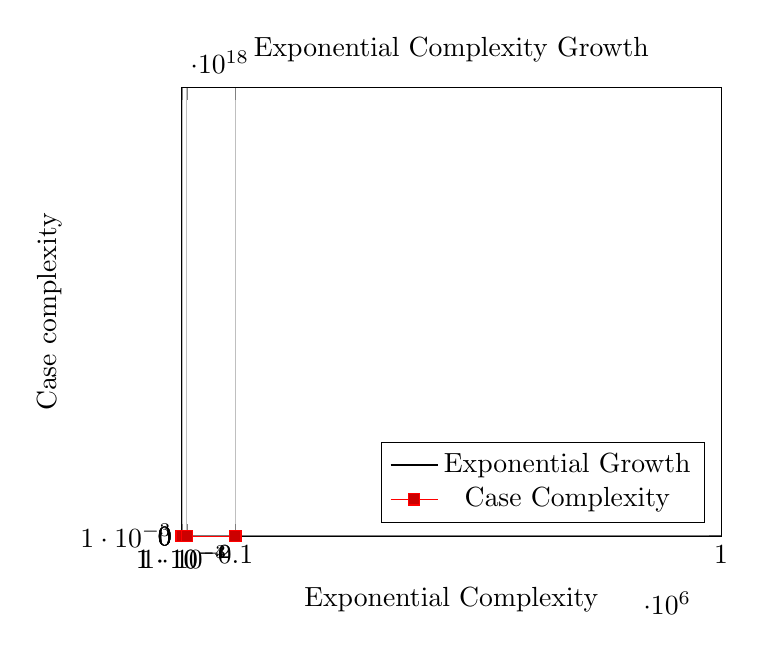
\begin{tikzpicture}
\begin{axis}[
    title={Exponential Complexity Growth},
    xlabel={Exponential Complexity},
    ylabel={Case complexity},
    xmin=0, xmax=1000000,
    ymin=0, ymax=1000000000000000000,
    log basis x=10,
    log basis y=10,
    xtick={100, 1000, 10000, 100000, 1000000},
    ytick={10^0, 10^3, 10^4, 10^7, 10^10, 10^15, 10^20},
    legend pos=south east,
    ymajorgrids=true,
    xmajorgrids=true,
]
\addplot[domain=1:1000000, samples=100] {x^2};
\addlegendentry{Exponential Growth};
\addplot coordinates {
(100, 10^3)
(10000, 10^7)
(100000, 10^10)
};
\addlegendentry{Case Complexity};
\node[anchor=north west] at (axis cs:100, 10^3) {100};
\node[anchor=north west] at (axis cs:10000, 10^7) {10K};
\node[anchor=north west] at (axis cs:100000, 10^10) {100K};
\node[anchor=north west] at (axis cs:1000000, 10^15) {1M};
\node[anchor=north west] at (axis cs:100, 10^3) {Car repair diagnosis};
\node[anchor=north west] at (axis cs:10000, 10^7) {Deep space mission control};
\node[anchor=north west] at (axis cs:100000, 10^10) {Chess (20 steps deep)};
\node[anchor=north west] at (axis cs:1000000, 10^15) {Military Logistics};
\node[anchor=north west] at (axis cs:1000000, 10^15) {VLSI Verification};
\node[anchor=north west] at (axis cs:1000000, 10^15) {War Gaming};
\end{axis}
\end{tikzpicture}

\textbf{No. of atoms} on the earth \quad $10^{30}$
\textbf{Seconds until} heat death of sun \quad $10^{47}$
\textbf{Protein folding} Calculation (petaflop-year) \quad $10^{30}$
\textbf{Variables} \quad Rules (Constraints)
\textbf{Credit:} Kumar, DARPA; cited in Computer World magazine
%
\subsection{Description}%
This slide, from a lecture on Artificial Intelligence Basics, graphically illustrates the challenge of exponential complexity growth in problem-solving.  It presents a graph with logarithmic scales on both the x-axis (representing exponential complexity) and the y-axis (representing case complexity).  The graph shows a steep upward trend, highlighting how the computational resources required to solve problems increase dramatically as the problem size grows.  The x-axis is labeled with increasing powers of 10, representing different problem sizes.  The y-axis is also labeled with increasing powers of 10, representing the computational resources needed.  The graph visually demonstrates the exponential relationship between problem size and computational cost.  The slide also lists several examples of real-world problems, such as car repair diagnosis, deep space mission control, chess, military logistics, VLSI verification, and war gaming, each with its corresponding estimated complexity (e.g., 100, 10K, 100K, 1M, etc.).  These examples are used to illustrate the exponential growth in complexity across various domains.  The slide also includes a note indicating that the estimates are rough and are for propositional reasoning.  The context of the course suggests that the slide is intended to highlight the limitations of current computational resources in tackling problems with high complexity, which is a key challenge in AI.%
\subsection{Figures}%
\begin{figure}[H]%
\centering%
\begin{subfigure}[b]{0.15\textwidth}%
\centering%

\includegraphics[width=\textwidth]{/Users/ashoksaravanan/Coding/ScribeLec/server/output/CS 243/lectures/15L2-SAT/figures/4.1.png}%
\caption{}%
\end{subfigure}%
\hspace{0.05\textwidth}%
\begin{subfigure}[b]{0.15\textwidth}%
\centering%

\includegraphics[width=\textwidth]{/Users/ashoksaravanan/Coding/ScribeLec/server/output/CS 243/lectures/15L2-SAT/figures/4.2.png}%
\caption{}%
\end{subfigure}%
\hspace{0.05\textwidth}%
\begin{subfigure}[b]{0.15\textwidth}%
\centering%

\includegraphics[width=\textwidth]{/Users/ashoksaravanan/Coding/ScribeLec/server/output/CS 243/lectures/15L2-SAT/figures/4.3.png}%
\caption{}%
\end{subfigure}%
\hspace{0.05\textwidth}%
\begin{subfigure}[b]{0.15\textwidth}%
\centering%

\includegraphics[width=\textwidth]{/Users/ashoksaravanan/Coding/ScribeLec/server/output/CS 243/lectures/15L2-SAT/figures/4.4.png}%
\caption{}%
\end{subfigure}%
\hspace{0.05\textwidth}%
\begin{subfigure}[b]{0.15\textwidth}%
\centering%

\includegraphics[width=\textwidth]{/Users/ashoksaravanan/Coding/ScribeLec/server/output/CS 243/lectures/15L2-SAT/figures/4.5.png}%
\caption{}%
\end{subfigure}%
\end{figure}

%
\newpage%
\section{Slide 5}%
\label{sec:Slide5}%
\subsection{Content}%

\textbf{Progress in the Last 20 Years}

\textbf{Focus:} Combinatorial Search Spaces, specifically, the Boolean satisfiability problem, SAT

\textbf{Significant progress since the 1990's.} How much?

\begin{itemize}
    \item \textbf{Problem size:} We went from 100 variables, 200 constraints (early 90's) to 1,000,000+ variables and 5,000,000+ constraints in 20 years
\end{itemize}

\textbf{Search space:} from $10^{30}$ to $10^{300,000}$. [Aside: "one can encode quite a bit in 1M variables."]

Is this just Moore's Law? It helped, but not much...

\begin{itemize}
    \item 2x faster computers does not mean can solve 2x larger instances
    \item search difficulty does not scale linearly with problem size!
\end{itemize}

\textbf{Tools:} 50+ competitive SAT solvers available
%
\subsection{Description}%
This slide, likely from a presentation or lecture on Artificial Intelligence Basics, discusses the progress made in solving the Boolean satisfiability problem (SAT) over the past 20 years.  It highlights the significant increase in problem size, from a few hundred variables and constraints in the early 1990s to millions of variables and constraints.  The slide emphasizes that the search space has expanded dramatically, from $10^{30}$ to $10^{300,000}$.  This exponential growth in search space is contrasted with the observation that faster computers don't necessarily translate to solving proportionally larger instances of the problem.  The difficulty of the problem does not scale linearly with the problem size.  The slide concludes by mentioning the availability of numerous competitive SAT solvers, suggesting that the progress is not solely due to hardware improvements but also to advancements in algorithms and software tools.%
\subsection{Figures}%
\begin{figure}[H]%
\centering%
\end{figure}

%
\newpage%
\section{Slide 6}%
\label{sec:Slide6}%
\subsection{Content}%
%
\subsection{Description}%
This slide, from a lecture on Artificial Intelligence Basics, discusses the size of bounded model checking (BMC) problems.  It introduces BMC as a problem in formal methods, specifically focused on checking if a given model (often a hardware design) satisfies a temporal property within a certain path length.  The slide states that BMC problems can be efficiently reduced to propositional satisfiability (SAT) problems.  Importantly, it highlights that if the property to be checked is an invariant, the BMC problem has a structure similar to many AI planning problems.  The reference [BCCZ99] indicates a specific publication related to BMC.  The slide's title, "How Large are the Problems?", suggests the discussion is about the computational complexity of these problems, and the text implies that the size of these problems can be substantial.%
\subsection{Figures}%
\begin{figure}[H]%
\centering%
\end{figure}

%
\newpage%
\section{Slide 7}%
\label{sec:Slide7}%
\subsection{Content}%
%
\subsection{Description}%
This slide presents a SAT (Boolean satisfiability) encoding.  It's likely part of a larger problem description, possibly from a formal methods or automated reasoning course.  The slide shows a set of clauses in the Conjunctive Normal Form (CNF) format, which is a standard way to represent Boolean formulas.  Each line represents a clause, with numbers representing literals (variables or their negations).  Positive numbers represent variables (e.g., x1, x7), and negative numbers represent negated variables (e.g., -x1).  The "p cnf 51639 368352" line indicates the problem type (CNF), the number of variables (51639), and the number of clauses (368352).  The example clauses, like ((not x1) or x7), illustrate how the problem is encoded.  The slide also explicitly states that x1, x2, x3, etc., are Boolean variables that need to be assigned True or False values.  The final question, "Should x1 be set to False??", suggests that the goal is to find a satisfying assignment for the given CNF formula, and x1 is a variable of particular interest.  The ellipsis (...) at the end of the clause list indicates that there are more clauses not shown on the slide. The context of the course (Artificial Intelligence Basics) suggests that the slide is about using SAT solvers to solve problems that can be encoded in this format.%
\subsection{Figures}%
\begin{figure}[H]%
\centering%
\end{figure}

%
\newpage%
\section{Slide 8}%
\label{sec:Slide8}%
\subsection{Content}%
%
\subsection{Description}%
This slide, likely from a lecture on Boolean Satisfiability (SAT) or a related topic in Artificial Intelligence Basics, displays a portion of a SAT problem encoding.  The numbers represent literals (variables or their negations) within a Conjunctive Normal Form (CNF) formula.  For example, "185 -9 0" likely represents the clause (x185 or not x9).  The numbers 177, 169, etc., are likely variable indices.  The notation "i.e., (x177 or x169 or x161 or x153 ... x33 or x25 or x17 or x9 or x1 or (not x185))" indicates an example of a clause, showing how multiple literals are combined using the logical OR operator.  The presence of negated variables (e.g., -185) further confirms this.  The phrase "clauses / constraints are getting more interesting..." suggests that the problem size and complexity are increasing, and the clauses are becoming more intricate.  The "Note x1 ..." at the end implies that x1 is a variable of particular importance or focus in this part of the problem.  The context of the course is crucial for understanding the specific meaning of the numbers and the overall problem being represented.%
\subsection{Figures}%
\begin{figure}[H]%
\centering%
\end{figure}

%
\newpage%
\section{Slide 9}%
\label{sec:Slide9}%
\subsection{Content}%
%
\subsection{Description}%
This slide, likely from a lecture on Boolean Satisfiability (SAT) or a related topic in Artificial Intelligence Basics, displays a large list of numbers.  The numbers represent literals (variables or their negations) within a Conjunctive Normal Form (CNF) formula.  The format is a sequence of integers, likely representing clauses in a SAT problem encoding.  For example, "10236 -10050 0" likely represents a clause (x10236 or not x10050).  The numbers are in the thousands, indicating a very large problem instance.  The presence of negative numbers (e.g., -10050) confirms that negated variables are included.  The "..." at the end indicates that the list continues beyond what is shown on the slide.  The context of the course (Artificial Intelligence Basics) suggests that the slide is about the representation and potential size of SAT problems, which are frequently encountered in AI, particularly in formal verification and planning. The sheer number of clauses (and variables) implies a complex problem that would require sophisticated algorithms and potentially significant computational resources to solve.%
\subsection{Figures}%
\begin{figure}[H]%
\centering%
\end{figure}

%
\newpage%
\section{Slide 10}%
\label{sec:Slide10}%
\subsection{Content}%

Finally 15,000 Pages Later
\begin{itemize}
    \item -7 260 0
    \item 7 -260 0
    \item 1072 1070 0
    \item -15 -14 -13 -12 -11 -10 0
    \item -15 -14 -13 -12 -11 10 0
    \item -15 -14 -13 -12 11 -10 0
    \item -15 -14 -13 -12 11 10 0
    \item -7 -6 -5 -4 -3 -2 0
    \item -7 -6 -5 -4 -3 2 0
    \item -7 -6 -5 -4 3 -2 0
    \item -7 -6 -5 -4 3 2 0
    \item 185 0
\end{itemize}
Search space of truth assignments:
$2^{50000} \approx 3.160699437 \cdot 10^{15051}$
Current SAT solvers solve this instance in just a few seconds!
%
\subsection{Description}%
This slide, likely from a lecture on Boolean Satisfiability (SAT) in an Artificial Intelligence Basics course, presents a large instance of a SAT problem.  The slide displays a list of clauses in Conjunctive Normal Form (CNF). Each line represents a clause, with integers representing literals (variables or their negations).  Positive integers represent variables, and negative integers represent negated variables.  For example, the line "-7 260 0" represents the clause (-x7 or x260 or x0).  The sheer number of clauses (and the large exponents in the search space calculation) indicates a very large and complex SAT problem.  The slide also highlights the efficiency of modern SAT solvers in handling such instances. The context of the course suggests that the slide is illustrating the practical application of SAT solvers to solve problems that can be encoded in this format, and the computational resources required to solve such problems. The phrase "Finally 15,000 Pages Later" implies that this is a significant step in a larger discussion or presentation, possibly about the limitations of traditional methods and the power of modern algorithms.%
\subsection{Figures}%
\begin{figure}[H]%
\centering%
\end{figure}

%
\newpage%
\section{Slide 11}%
\label{sec:Slide11}%
\subsection{Content}%

SAT Solvers as Search Engines
Systematic SAT solvers have become really efficient at searching fast
E.g., on an IBM model checking instance from SAT Race 2006, with $\sim$170k variables,
725k clauses, solvers such as MiniSat and RSat roughly:
\begin{itemize}
    \item Make & 2000-5000 decisions/second \\
    \item Deduce & 600-1000 conflicts/second \\
    \item Learn & 600-1000 clauses/second (\#clauses grows rapidly) \\
    \item Restart & every 1-2 seconds (aggressive restarts)
\end{itemize}
%
\subsection{Description}%
This slide, from a lecture on Artificial Intelligence Basics, discusses the efficiency of modern SAT solvers.  It highlights the performance of solvers like MiniSat and RSat on a specific instance of an IBM model checking problem from SAT Race 2006.  The problem has approximately 170,000 variables and 725,000 clauses.  The slide presents performance metrics for different solver operations:  "Make" operations (decisions/second), "Deduce" operations (conflicts/second), "Learn" operations (clauses/second), and "Restart" frequency (every 1-2 seconds).  The context of the course suggests that the slide is illustrating the speed and efficiency of modern SAT solvers in handling large-scale problems, which are common in various AI applications. The notation $\sim$170k indicates an approximate value of 170,000 variables. The phrase "#clauses grows rapidly" suggests that the number of clauses learned by the solver increases during the search process, which is a common characteristic of SAT solvers.%
\subsection{Figures}%
\begin{figure}[H]%
\centering%
\end{figure}

%
\newpage%
\section{Slide 12}%
\label{sec:Slide12}%
\subsection{Content}%

\begin{tabular}{ |l|c|c|c|c| } 
 \hline
 Instance & Posit' 94 & Grasp' 96 & Sato' 98 & Chaff' 01 \\ 
 \hline
 ssa2670-136 & 40.66s & 1.20s & 0.95s & 0.02s \\ 
 bf1355-638 & 1805.21s & 0.11s & 0.04s & 0.01s \\ 
 pret150\_25 & >3000s & 0.21s & 0.09s & 0.01s \\ 
 dubois100 & >3000s & 11.85s & 0.08s & 0.01s \\ 
 aim200-2\_0-no-1 & >3000s & 0.01s & < 0.01s & < 0.01s \\ 
 2dlx\_...\_bug005 & >3000s & >3000s & >3000s & 2.90s \\ 
 c6288 & >3000s & >3000s & >3000s & >3000s \\ 
 \hline
\end{tabular}
Solvers have continually improved over time
\newline
Source: MarquesSilva-02
%
\subsection{Description}%
This slide, from a lecture on Artificial Intelligence Basics, presents a table summarizing the performance of different SAT solvers on various problem instances.  The table shows the time taken (in seconds) by different solvers (Posit' 94, Grasp' 96, Sato' 98, and Chaff' 01) to solve each instance.  The instances are named (e.g., ssa2670-136, bf1355-638).  The time values are presented in a tabular format.  A value of ">3000s" indicates that the solver took more than 3000 seconds to solve the instance.  The table shows the progress of SAT solvers over time, with newer solvers (like Chaff' 01) being significantly faster than older ones (like Posit' 94) on many instances.  The context of the course suggests that the slide is illustrating the evolution of SAT solver technology and the improvement in their efficiency over time. The "Source" indicates the origin of the data, which is likely a research paper or benchmark dataset.%
\subsection{Figures}%
\begin{figure}[H]%
\centering%
\end{figure}

%
\newpage%
\section{Slide 13}%
\label{sec:Slide13}%
\subsection{Content}%

Satisfiability of a CNF formula
\begin{itemize}
    \item Notations
    \begin{itemize}
        \item Let $C_1, \dots, C_m$ be clauses over a finite set $V$ of Boolean variables $p_1, \dots, p_n$.
        \item Define $\phi = C_1 \land \dots \land C_m$.
        \item Let $v$ be an assignment on $V$.
    \end{itemize}
    \item Observations
    \begin{itemize}
        \item The CNF formula $\phi$ is satisfiable by $v$ if, and only if, the clause $C_i$, for all $i \in \{1, \dots, m\}$, is satisfiable by $v$.
        \item A clause $C_i$, for some $i \in \{1, \dots, m\}$, is satisfiable by $v$ if, and only if, at least one of its literals evaluates to true by $v$.
    \end{itemize}
    \item Consequences
    \begin{itemize}
        \item To check whether or not $v$ satisfies $\phi$, we may not need to know the truth values of all literals in all clauses.
        \item For instance, if $v(p) = \text{true}$ and $v(q) = \text{false}$, we can see that the formula $(p \lor q \lor \neg r) \land (\neg q \lor s \lor q)$ is satisfied without considering $v(r)$ and $v(s)$.
    \end{itemize}
\end{itemize}
%
\subsection{Description}%
This slide, likely from a lecture on Artificial Intelligence Basics, defines and discusses the concept of satisfiability for a Conjunctive Normal Form (CNF) formula.  It introduces the notation for clauses ($C_1, \dots, C_m$), a finite set of Boolean variables ($p_1, \dots, p_n$), and a formula $\phi$ constructed as a conjunction of these clauses.  An assignment $v$ on the variables is also defined.  The slide then presents observations about satisfiability: a CNF formula is satisfiable by an assignment if and only if each clause is satisfiable by that assignment.  A clause is satisfiable if at least one of its literals evaluates to true under the assignment.  Crucially, the slide highlights a consequence: to determine if an assignment satisfies the formula, it might not be necessary to know the truth values of all literals in all clauses.  The example given demonstrates this by showing how the truth values of some variables (r and s) are irrelevant to the satisfiability of the formula if the truth values of p and q are known.  The context of the course suggests that this slide is part of a discussion on Boolean logic, SAT solvers, and how to efficiently check for satisfiability in CNF formulas.%
\subsection{Figures}%
\begin{figure}[H]%
\centering%
\end{figure}

%
\newpage%
\section{Slide 14}%
\label{sec:Slide14}%
\subsection{Content}%

Partial Assignment
A partial assignment on $V$ is a partial function that associates to some Boolean variables of $V$ a truth value (either \textit{true} or \textit{false}) and can be undefined for the others.
Under a partial assignment on $V$, a clause $C$ on $V$ can be
\begin{itemize}
    \item true if one of its literals is true,
    \item false (or conflicting) if all its literals are false,
    \item undefined (or unresolved) if it is neither true nor false.
\end{itemize}
Remarks
\begin{itemize}
    \item Partial assignments allow us to construct assignments for a set of clauses incrementally, that is, one clause after another.
    \item The SAT solving algorithms to be presented next use partial assignments.
    \item They all start with an empty assignment (that is, the truth values of all Boolean variables are not defined) and try to extend this assignment, assigning one Boolean variable after another.
\end{itemize}
%
\subsection{Description}%
This slide defines a "partial assignment" in the context of SAT (Satisfiability) problem solving.  A partial assignment is a function that assigns truth values (\textit{true} or \textit{false}) to some of the Boolean variables in a set $V$, leaving others undefined.  The slide then describes how a clause $C$ can be evaluated under a partial assignment:  it's \textit{true} if at least one literal in the clause is \textit{true}; \textit{false} if all literals are \textit{false}; and \textit{undefined} if neither of the previous conditions hold.  The "Remarks" section emphasizes the incremental nature of partial assignments in SAT solvers.  The solvers use partial assignments to build complete assignments step-by-step, starting with an empty assignment (no variables assigned) and progressively assigning values to variables.  The context of the course (Artificial Intelligence Basics) suggests that this slide is part of a discussion on SAT solvers and their strategies for finding satisfying assignments to Boolean formulas.%
\subsection{Figures}%
\begin{figure}[H]%
\centering%
\end{figure}

%
\newpage%
\section{Slide 15}%
\label{sec:Slide15}%
\subsection{Content}%

Simplification of a formula by an evaluated literal
For the CNF formula $\phi$ and a Boolean variables $p$, we denote by $\phi |_p$, the formula obtained from $\phi$ by replacing all occurrences of $p$ by true and simplifying the result by removing:
\begin{itemize}
    \item all true clauses,
    \item all false literals from undefined clauses.
\end{itemize}
The operation that maps $(\phi, p)$ to $\phi |_p$ is called the simplification of $\phi$ at $p$.
Similarly, we define $\phi |_{\neg p}$ as the formula obtained from $\phi$ by replacing all occurrences of $p$ by false and simplifying the result by removing:
\begin{itemize}
    \item all true clauses,
    \item all false literals from undefined clauses.
\end{itemize}
The operation that maps $(\phi, p)$ to $\phi |_{\neg p}$ is called the simplification of $\phi$ at $p$.
Example:
$\phi = (p \lor q \lor \neg r) \land (\neg p \lor \neg r) \implies \phi |_{\neg p} = q \lor \neg r$
%
\subsection{Description}%
This slide discusses the simplification of a Conjunctive Normal Form (CNF) formula $\phi$ based on the truth value of a Boolean variable $p$.  It defines two operations: $\phi |_p$ and $\phi |_{\neg p}$.  $\phi |_p$ is the simplified formula obtained by setting $p$ to true in $\phi$ and removing any clauses that become trivially true, and any literals that become false.  $\phi |_{\neg p}$ is similarly obtained by setting $p$ to false.  The example demonstrates how these simplifications work on a specific CNF formula.  The context of the course (Artificial Intelligence Basics) suggests that this slide is part of a discussion on SAT (Satisfiability) solvers and techniques for efficiently evaluating and simplifying Boolean formulas.%
\subsection{Figures}%
\begin{figure}[H]%
\centering%
\end{figure}

%
\newpage%
\section{Slide 16}%
\label{sec:Slide16}%
\subsection{Content}%

\textbf{Simplification of a formula by an evaluated literal}

\textbf{Proposition}
For $\phi$ and $p$ as in the above definition, we have:
\begin{itemize}
    \item if $\phi|_p$ is satisfiable, then $\phi$ is satisfiable too,
    \item if $\phi|_{\neg p}$ is satisfiable, then $\phi$ is satisfiable too.
    \item if $\phi$ is satisfiable then either $\phi|_p$ or $\phi|_{\neg p}$ is satisfiable.
\end{itemize}

\textbf{Remarks}
The above proposition is a key argument in the SAT solving algorithms to be presented hereafter.
The proof of this proposition is easy and left as an exercise.
%
\subsection{Description}%
This slide presents a proposition related to simplifying a CNF formula ($\phi$) based on the truth value of a variable ($p$).  It states three conditions: 1) If the formula $\phi$ simplified by setting $p$ to true ($\phi|_p$) is satisfiable, then the original formula $\phi$ is also satisfiable. 2) If the formula $\phi$ simplified by setting $p$ to false ($\phi|_{\neg p}$) is satisfiable, then the original formula $\phi$ is also satisfiable. 3) If the original formula $\phi$ is satisfiable, then either the simplified formula with $p$ set to true or the simplified formula with $p$ set to false must be satisfiable.  The "Remarks" section indicates that this proposition is a crucial step in SAT solving algorithms, and the proof is omitted.  The context of the course (Artificial Intelligence Basics) suggests that this slide is part of a discussion on SAT solvers and their strategies for finding satisfying assignments to Boolean formulas.%
\subsection{Figures}%
\begin{figure}[H]%
\centering%
\end{figure}

%
\newpage%
\section{Slide 17}%
\label{sec:Slide17}%
\subsection{Content}%

\textbf{Principles of SAT solving algorithms}

The SAT solving algorithms presented hereafter are based on the following ideas:

First, each algorithm is stated as a recursive function taking a propositional formula $\phi$ and a partial assignment $v$ as arguments.

Second, these functions may modify their arguments:
\begin{itemize}
    \item the partial assignment $v$ can be extended,
    \item the formula $\phi$ can be simplified at the newly assigned literal.
\end{itemize}

Third, before extending the assignment $v$ and simplifying the formula $\phi$, the function checks whether $\phi$ can be proved to be true or false, whatever are the values of the remaining unassigned Boolean variables.
%
\subsection{Description}%
This slide outlines the principles behind SAT (Satisfiability) solving algorithms.  It states that each algorithm is a recursive function that takes a propositional formula ($\phi$) and a partial assignment ($v$) as input.  Crucially, the function can modify both its arguments:  the partial assignment can be extended (by assigning a truth value to a previously unassigned variable), and the formula itself can be simplified by considering the newly assigned literal.  Importantly, before making any changes, the algorithm checks if the formula is already definitively true or false, given the current partial assignment.  This is a key optimization step in SAT solvers, as it can avoid unnecessary work if a formula is immediately determined to be unsatisfiable or satisfiable. The context of the course (Artificial Intelligence Basics) suggests that this slide is part of a lecture on SAT solvers and their strategies for finding satisfying assignments to Boolean formulas.%
\subsection{Figures}%
\begin{figure}[H]%
\centering%
\end{figure}

%
\newpage%
\section{Slide 18}%
\label{sec:Slide18}%
\subsection{Content}%

\textbf{Naïve Solver}

\textbf{Input:} A propositional formula $\phi$ on a finite set $V$ and a partial assignment $v$ on $V$ such that only variables unassigned by $v$ occur in $\phi$.

\textbf{Output:} true if $\phi$ is satisfiable, false otherwise.

\textbf{Naive\_SAT($\phi$, $v$)} \{
\begin{itemize}
    \item if every clause of $\phi$ has a true literal, return true;
    \item if any clause of $\phi$ has all false literals, return false;
    \item choose an $p \in V$ that is unassigned in $v$;
    \item assign $p$ to true, that is, let $v(p)$ = true;
    \item if Naive\_SAT($\phi|_p$, $v$) returns true, then return true;  \# this is a recursive call
    \item assign $p$ to false, that is, let $v(p)$ = false;
    \item if Naive\_SAT($\phi|_{\neg p}$, $v$) returns true, then return true;  \# this is a recursive call
    \item unassign $v(p)$; \# backtracking takes place here
    \item return false;
\end{itemize}
\}
%
\subsection{Description}%
This slide presents a recursive algorithm called `Naive_SAT` for solving the Satisfiability (SAT) problem.  The input is a propositional formula ($\phi$) defined over a set of variables ($V$) and a partial assignment ($v$) to some of those variables.  The algorithm aims to determine if there exists a complete assignment to all variables in $V$ that satisfies the formula $\phi$.  The `Naive_SAT` function recursively explores possible assignments.  It first checks if the formula is already trivially satisfiable (every clause has a true literal) or unsatisfiable (every clause has all false literals). If neither of these conditions holds, it selects an unassigned variable ($p$) and explores two possibilities: assigning $p$ to true and recursively calling `Naive_SAT` with the simplified formula ($\phi|_p$) and the updated assignment; or assigning $p$ to false and recursively calling `Naive_SAT` with the simplified formula ($\phi|_{\neg p}$) and the updated assignment.  If either recursive call returns `true`, the algorithm returns `true`.  If both recursive calls return `false`, the algorithm backtracks by resetting the assignment for $p$ and returns `false`.  The algorithm's structure is a depth-first search approach to explore all possible assignments. The context of the course (Artificial Intelligence Basics) suggests that this slide is part of a lecture on SAT solvers and their strategies for finding satisfying assignments to Boolean formulas.%
\subsection{Figures}%
\begin{figure}[H]%
\centering%
\begin{subfigure}[b]{0.15\textwidth}%
\centering%

\includegraphics[width=\textwidth]{/Users/ashoksaravanan/Coding/ScribeLec/server/output/CS 243/lectures/15L2-SAT/figures/18.1.png}%
\caption{}%
\end{subfigure}%
\end{figure}

%
\newpage%
\section{Slide 19}%
\label{sec:Slide19}%
\subsection{Content}%

\textbf{The Pure Literal Rule}

Given a propositional CNF formula $\phi$ for which we check whether $\phi$ is satisfiable or not, if a variable is always positive (that is, never appears with a $\neg$) or always negative (that is, always appears with a $\neg$) in $\phi$, one only needs to set it to one value: true for positive variables, false for negative variables.

Such variables are called pure.
%
\subsection{Description}%
This slide introduces the "Pure Literal Rule" in the context of SAT (Satisfiability) solving algorithms.  It states that if a variable in a Conjunctive Normal Form (CNF) formula ($\phi$) always appears positively (without a negation symbol) or always appears negatively (with a negation symbol), then the algorithm can immediately assign a truth value to that variable.  If the variable is always positive, it's assigned true; if it's always negative, it's assigned false.  These variables are called "pure" because their truth value is uniquely determined by their presence in the formula.  This rule is a simplification technique used to reduce the search space in SAT solvers, as it eliminates the need to explore different assignments for these variables. The context of the course (Artificial Intelligence Basics) suggests that this slide is part of a lecture on SAT solvers and their strategies for finding satisfying assignments to Boolean formulas.%
\subsection{Figures}%
\begin{figure}[H]%
\centering%
\end{figure}

%
\newpage%
\section{Slide 20}%
\label{sec:Slide20}%
\subsection{Content}%

\textbf{Unit Propagation}

Unit propagation (a.k.a Boolean constraint propagation or BCP) is a key component to fast SAT solving.
\begin{itemize}
    \item Whenever all the literals in a clause are false except one, the remaining literal must be true in any satisfying assignment; such a clause is called a unit clause.
    \item Therefore, the algorithm can assign it to true immediately.
    \item After assigning a variable, there are often many unit clauses.
    \item Setting a literal in a unit clause often creates other unit clauses, leading to a cascade.
\end{itemize}

Based on those observations, we define a sub-algorithm BCP as follows.

BCP($\phi$, $v$)
\begin{itemize}
    \item Repeatedly search for unit clauses, and set unassigned literal to required value.
    \item If a literal is assigned to a conflicting value, then return false else return true.
\end{itemize}
%
\subsection{Description}%
This slide describes the Unit Propagation algorithm, a crucial component of SAT (Satisfiability) solvers.  It explains that when all literals in a clause are false except one, the remaining literal must be true. This is called a "unit clause."  The algorithm can immediately assign the remaining literal to true.  The key point is that assigning a variable can create more unit clauses, leading to a cascading effect.  The slide then defines a sub-algorithm, BCP ($\phi$, $v$), which repeatedly searches for unit clauses and assigns the unassigned literals in those clauses to their required values.  If an assignment leads to a conflict (a literal is assigned a value that contradicts the formula), the algorithm returns false; otherwise, it returns true.  The context of the course (Artificial Intelligence Basics) suggests that this slide is part of a lecture on SAT solvers and their strategies for finding satisfying assignments to Boolean formulas.%
\subsection{Figures}%
\begin{figure}[H]%
\centering%
\end{figure}

%
\newpage%
\section{Slide 21}%
\label{sec:Slide21}%
\subsection{Content}%

\textbf{Davis-Putnam-Logemann-Loveland (DPLL) Algorithm}

\textbf{Input:} A propositional formula $\phi$ on a finite set $V$ and a partial assignment $v$ on $V$ such that only variables unassigned by $v$ occur in $\phi$.

\textbf{Output:} true if $\phi$ is satisfiable, false otherwise.

DPLL($\phi$, $v$) \{
\begin{itemize}
    \item if every clause of $\phi$ has a true literal, return true;
    \item if any clause of $\phi$ has all false literals, return false;
    \item if BCP($\phi$, $v$) returns false, then return false;
    \item choose an $p \in V$ that is unassigned in $v$;
    \item assign $p$ to true, that is, let $v(p)$ = true;
    \item if DPLL($\phi|_p$, $v$) returns true, then return true;
    \item assign $p$ to false, that is, let $v(p)$ = false;
    \item if DPLL($\phi|_{\neg p}$, $v$) returns true, then return true;
    \item unassign $v(p)$;  \# backtracking takes place here
    \item return false;
\end{itemize}
\}
%
\subsection{Description}%
This slide presents the Davis-Putnam-Logemann-Loveland (DPLL) algorithm for solving the Satisfiability (SAT) problem.  The input is a propositional formula ($\phi$) defined over a set of variables ($V$) and a partial assignment ($v$) to some of those variables.  The algorithm recursively explores possible assignments to determine if a satisfying assignment exists.  It first checks for trivial cases: if every clause has a true literal, the formula is satisfiable; if any clause has all false literals, the formula is unsatisfiable.  It then uses Boolean Constraint Propagation (BCP) to simplify the formula. If BCP detects a conflict, the algorithm backtracks.  If neither of these conditions holds, it selects an unassigned variable ($p$) and explores two possibilities: assigning $p$ to true and recursively calling DPLL with the simplified formula ($\phi|_p$) and the updated assignment; or assigning $p$ to false and recursively calling DPLL with the simplified formula ($\phi|_{\neg p}$) and the updated assignment.  If either recursive call returns `true`, the algorithm returns `true`.  If both recursive calls return `false`, the algorithm backtracks by resetting the assignment for $p$ and returns `false`.  The algorithm's structure is a depth-first search approach to explore all possible assignments.  The context of the course (Artificial Intelligence Basics) suggests that this slide is part of a lecture on SAT solvers and their strategies for finding satisfying assignments to Boolean formulas.%
\subsection{Figures}%
\begin{figure}[H]%
\centering%
\begin{subfigure}[b]{0.15\textwidth}%
\centering%

\includegraphics[width=\textwidth]{/Users/ashoksaravanan/Coding/ScribeLec/server/output/CS 243/lectures/15L2-SAT/figures/21.1.png}%
\caption{}%
\end{subfigure}%
\end{figure}

%
\newpage%
\section{Slide 22}%
\label{sec:Slide22}%
\subsection{Content}%

\textbf{DPLL Search}

\begin{itemize}
    \item (a' + b + c)
    \item (a + c + d)
    \item (a + c + d')
    \item (a + c' + d)
    \item (a + c' + d')
    \item (b' + c' + d)
    \item (a' + b + c')
    \item (a' + b' + c)
\end{itemize}
%
\subsection{Description}%
This slide displays a set of clauses, likely part of a propositional logic formula.  Each clause is a disjunction (OR) of literals.  The literals are represented by variables (a, b, c, d) possibly negated (a', b', c', d').  The context of the slide suggests that this is a step in a Davis-Putnam-Logemann-Loveland (DPLL) algorithm, a backtracking search algorithm for determining the satisfiability of Boolean formulas.  The clauses are likely used to represent the constraints of the problem, and the algorithm would attempt to find an assignment of truth values to the variables that satisfies all the clauses.  The presence of the title "DPLL Search" confirms this interpretation.  The context of the course (Artificial Intelligence Basics) is crucial for understanding the role of these clauses in the SAT problem.%
\subsection{Figures}%
\begin{figure}[H]%
\centering%
\begin{subfigure}[b]{0.15\textwidth}%
\centering%

\includegraphics[width=\textwidth]{/Users/ashoksaravanan/Coding/ScribeLec/server/output/CS 243/lectures/15L2-SAT/figures/22.1.png}%
\caption{}%
\end{subfigure}%
\end{figure}

%
\newpage%
\section{Slide 23}%
\label{sec:Slide23}%
\subsection{Content}%
%
\subsection{Description}%
This slide, titled "DPLL Search," displays a set of clauses in a propositional logic formula.  Each clause is a disjunction (OR) of literals, where literals are variables (a, b, c, d) or their negations (a', b', c', d').  The clauses are likely part of a larger formula used in the Davis-Putnam-Logemann-Loveland (DPLL) algorithm, a backtracking search algorithm for determining the satisfiability of Boolean formulas.  A small circle labeled "a" and the arrow pointing to it from the origin (0) indicates a decision variable. The context of the course (Artificial Intelligence Basics) suggests that this slide is part of a lecture on SAT solvers and their strategies for finding satisfying assignments to Boolean formulas. The arrangement of the clauses in a list format suggests that the algorithm is considering these clauses in a specific order or during a specific step of the DPLL search process.%
\subsection{Figures}%
\begin{figure}[H]%
\centering%
\begin{subfigure}[b]{0.15\textwidth}%
\centering%

\includegraphics[width=\textwidth]{/Users/ashoksaravanan/Coding/ScribeLec/server/output/CS 243/lectures/15L2-SAT/figures/23.1.png}%
\caption{}%
\end{subfigure}%
\end{figure}

%
\newpage%
\section{Slide 24}%
\label{sec:Slide24}%
\subsection{Content}%
%
\subsection{Description}%
This slide presents a DPLL search, a backtracking algorithm for solving the satisfiability (SAT) problem.  It shows a set of clauses (disjunctions of literals) in a propositional logic formula.  The literals are variables (a, b, c, d) and their negations (a', b', c', d').  The slide also displays an implication graph.  The graph visually represents the relationships between variables and their assignments.  Nodes represent variables (a, b, c, d) and their assigned values (0 or 1).  Arrows indicate the implications between variables.  A red box labeled "0" is present, indicating a conflict detected during unit propagation.  The text "Unit propagation: Quickly determines conflicts!" highlights the role of unit propagation in the DPLL algorithm.  The implication graph shows that assigning a=0 and d=1 leads to a conflict, which is indicated by the "Conflict!" label.  The context of the course (Artificial Intelligence Basics) suggests that this slide is part of a lecture on SAT solvers and their strategies for finding satisfying assignments to Boolean formulas. The implication graph is crucial for understanding how the algorithm determines conflicts and backtracks.%
\subsection{Figures}%
\begin{figure}[H]%
\centering%
\begin{subfigure}[b]{0.15\textwidth}%
\centering%

\includegraphics[width=\textwidth]{/Users/ashoksaravanan/Coding/ScribeLec/server/output/CS 243/lectures/15L2-SAT/figures/24.1.png}%
\caption{}%
\end{subfigure}%
\hspace{0.05\textwidth}%
\begin{subfigure}[b]{0.15\textwidth}%
\centering%

\includegraphics[width=\textwidth]{/Users/ashoksaravanan/Coding/ScribeLec/server/output/CS 243/lectures/15L2-SAT/figures/24.2.png}%
\caption{}%
\end{subfigure}%
\end{figure}

%
\newpage%
\section{Slide 25}%
\label{sec:Slide25}%
\subsection{Content}%

\textbf{DPLL Search}

\begin{itemize}
    \item (a' + b + c)
    \item (a + c + d)
    \item (a + c + d')
    \item (a + c' + d)
    \item (a + c' + d')
    \item (b' + c' + d)
    \item (a' + b + c')
    \item (a' + b' + c)
\end{itemize}

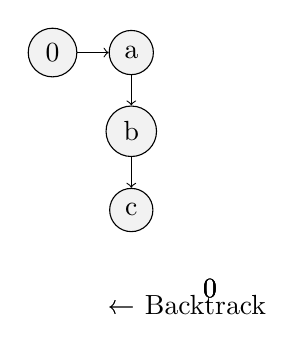
\begin{tikzpicture}[node distance=1cm]
    \node[circle, draw, fill=lightgray!20] (root) {0};
    \node[circle, draw, fill=lightgray!20, right of=root] (a) {a};
    \node[circle, draw, fill=lightgray!20, below of=a] (b) {b};
    \node[circle, draw, fill=lightgray!20, below of=b] (c) {c};
    \draw[->] (root) -- (a);
    \draw[->] (a) -- (b);
    \draw[->] (b) -- (c);
    \node[below of=c, xshift=1cm] {0};
    \node[below of=c, xshift=1cm] {0};
    \node[below of=c, xshift=1cm] {0};
    \node[below of=c, xshift=1cm, red, rectangle, minimum width=1cm, minimum height=0.5cm] {};
    \node[below right of=c, yshift=-0.5cm] {← Backtrack};
\end{tikzpicture}
%
\subsection{Description}%
This slide, titled "DPLL Search," presents a set of clauses in a propositional logic formula.  Each clause is a disjunction (OR) of literals, where literals are variables (a, b, c, d) or their negations (a', b', c', d').  The clauses are likely part of a larger formula used in the Davis-Putnam-Logemann-Loveland (DPLL) algorithm, a backtracking search algorithm for determining the satisfiability of Boolean formulas.  The clauses are listed in a bulleted list.  A tree diagram is also shown, visually representing the search space explored by the DPLL algorithm.  The nodes in the tree represent variable assignments.  The edges represent the choices made during the search.  The node labeled "c" has a "← Backtrack" label, indicating that the algorithm backtracked from this assignment.  A red rectangle is positioned below the "c" node, suggesting a conflict or failure to satisfy the clauses at that point in the search.  The context of the course (Artificial Intelligence Basics) suggests that this slide is part of a lecture on SAT solvers and their strategies for finding satisfying assignments to Boolean formulas. The tree diagram is crucial for understanding the backtracking nature of the DPLL algorithm and how it explores different possibilities to find a solution.%
\subsection{Figures}%
\begin{figure}[H]%
\centering%
\begin{subfigure}[b]{0.15\textwidth}%
\centering%

\includegraphics[width=\textwidth]{/Users/ashoksaravanan/Coding/ScribeLec/server/output/CS 243/lectures/15L2-SAT/figures/25.1.png}%
\caption{}%
\end{subfigure}%
\hspace{0.05\textwidth}%
\begin{subfigure}[b]{0.15\textwidth}%
\centering%

\includegraphics[width=\textwidth]{/Users/ashoksaravanan/Coding/ScribeLec/server/output/CS 243/lectures/15L2-SAT/figures/25.2.png}%
\caption{}%
\end{subfigure}%
\end{figure}

%
\newpage%
\section{Slide 26}%
\label{sec:Slide26}%
\subsection{Content}%

\textbf{DPLL Search}

\begin{itemize}
    \item (a' + b + c)
    \item (a + c + d)
    \item (a + c + d')
    \item (a + c' + d)
    \item (a + c' + d')
    \item (b' + c' + d)
    \item (a' + b + c')
    \item (a' + b' + c)
\end{itemize}

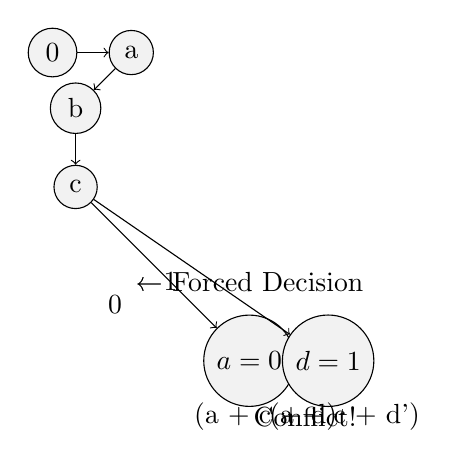
\begin{tikzpicture}[node distance=1cm]
    \node[circle, draw, fill=lightgray!20] (root) {0};
    \node[circle, draw, fill=lightgray!20, right of=root] (a) {a};
    \node[circle, draw, fill=lightgray!20, below left of=a] (b) {b};
    \node[circle, draw, fill=lightgray!20, below of=b] (c) {c};
    \draw[->] (root) -- (a);
    \draw[->] (a) -- (b);
    \draw[->] (b) -- (c);
    \node[below of=c, xshift=0.5cm, yshift=-0.5cm] {0};
    \node[below of=c, xshift=0.5cm, yshift=-0.5cm, red, rectangle, minimum width=1cm, minimum height=0.5cm] {};
    \node[below right of=c, yshift=-0.5cm, xshift=0.5cm] {1};
    \node[below right of=c, yshift=-0.5cm, xshift=1.5cm] {← Forced Decision};
    \node[below right of=c, yshift=-1.5cm, xshift=1.5cm, circle, draw, fill=lightgray!20] (a0) {$a=0$};
    \node[below right of=c, yshift=-1.5cm, xshift=2.5cm, circle, draw, fill=lightgray!20] (d1) {$d=1$};
    \node[below right of=d1, xshift=-1cm] {Conflict!};
    \draw[->] (c) -- (a0);
    \draw[->] (c) -- (d1);
    \node[below right of=a0, xshift=-0.5cm] {(a + c + d)};
    \node[below right of=d1, xshift=-0.5cm] {(a + c + d')};
\end{tikzpicture}
%
\subsection{Description}%
This slide displays a DPLL search, a backtracking algorithm for solving the satisfiability (SAT) problem.  It shows a set of clauses (disjunctions of literals) in a propositional logic formula.  The literals are variables (a, b, c, d) and their negations (a', b', c', d').  The clauses are listed in a bulleted list above the tree diagram.  The tree diagram visually represents the search space explored by the DPLL algorithm.  The nodes in the tree represent variable assignments.  The edges represent the choices made during the search.  The node labeled "c" has a "1 ← Forced Decision" label, indicating that the algorithm made a forced decision for variable c.  A red rectangle is positioned below the "c" node, suggesting a conflict or failure to satisfy the clauses at that point in the search.  Below the "c" node, the slide shows the assignments a=0 and d=1, which led to a conflict, indicated by the "Conflict!" label.  The context of the course (Artificial Intelligence Basics) suggests that this slide is part of a lecture on SAT solvers and their strategies for finding satisfying assignments to Boolean formulas. The tree diagram is crucial for understanding the backtracking nature of the DPLL algorithm and how it explores different possibilities to find a solution. The clauses below the tree diagram show the constraints that led to the conflict.%
\subsection{Figures}%
\begin{figure}[H]%
\centering%
\begin{subfigure}[b]{0.15\textwidth}%
\centering%

\includegraphics[width=\textwidth]{/Users/ashoksaravanan/Coding/ScribeLec/server/output/CS 243/lectures/15L2-SAT/figures/26.1.png}%
\caption{}%
\end{subfigure}%
\hspace{0.05\textwidth}%
\begin{subfigure}[b]{0.15\textwidth}%
\centering%

\includegraphics[width=\textwidth]{/Users/ashoksaravanan/Coding/ScribeLec/server/output/CS 243/lectures/15L2-SAT/figures/26.2.png}%
\caption{}%
\end{subfigure}%
\hspace{0.05\textwidth}%
\begin{subfigure}[b]{0.15\textwidth}%
\centering%

\includegraphics[width=\textwidth]{/Users/ashoksaravanan/Coding/ScribeLec/server/output/CS 243/lectures/15L2-SAT/figures/26.3.png}%
\caption{}%
\end{subfigure}%
\end{figure}

%
\newpage%
\section{Slide 27}%
\label{sec:Slide27}%
\subsection{Content}%

\textbf{DPLL Search}

\begin{itemize}
    \item (a' + b + c)
    \item (a + c + d)
    \item (a + c + d')
    \item (a + c' + d)
    \item (a + c' + d')
    \item (b' + c' + d)
    \item (a' + b + c')
    \item (a' + b' + c)
\end{itemize}

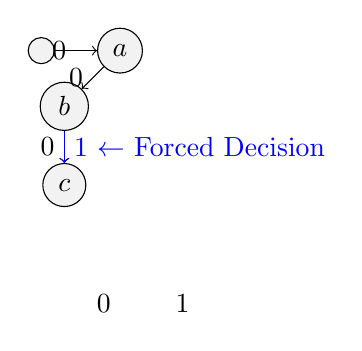
\begin{tikzpicture}[node distance=1cm]
    \node[circle, draw, fill=lightgray!20] (root) {};
    \node[circle, draw, fill=lightgray!20, right of=root] (a) {$a$};
    \node[circle, draw, fill=lightgray!20, below left of=a] (b) {$b$};
    \node[circle, draw, fill=lightgray!20, below of=b] (c) {$c$};
    \draw[->] (root) -- (a) node[midway, left] {0};
    \draw[->] (a) -- (b) node[midway, left] {0};
    \draw[->] (b) -- (c) node[midway, left] {0};
    \draw[->, blue] (b) -- (c) node[midway, right] {1 $\leftarrow$ Forced Decision};
    \node[below of=c, xshift=0.5cm, yshift=-0.5cm] {0};
    \node[below of=c, xshift=0.5cm, yshift=-0.5cm, red, rectangle, minimum width=1cm, minimum height=0.5cm] {};
    \node[below of=c, xshift=1.5cm, yshift=-0.5cm] {1};
\end{tikzpicture}
%
\subsection{Description}%
This slide, titled "DPLL Search," presents a portion of a search tree for the satisfiability (SAT) problem.  The problem is represented by a set of clauses (disjunctions of literals) in propositional logic.  The literals are variables (a, b, c, d) and their negations (a', b', c', d').  The clauses are listed in a bulleted list above the tree.  The tree diagram visually represents the search space explored by the DPLL algorithm.  The nodes in the tree represent variable assignments.  The edges represent the choices made during the search.  The node labeled "b" has a "1 ← Forced Decision" label, indicating that the algorithm made a forced decision for variable b.  A red rectangle is positioned below the "c" node, suggesting a conflict or failure to satisfy the clauses at that point in the search.  The context of the course (Artificial Intelligence Basics) suggests that this slide is part of a lecture on SAT solvers and their strategies for finding satisfying assignments to Boolean formulas. The tree diagram is crucial for understanding the backtracking nature of the DPLL algorithm and how it explores different possibilities to find a solution.  The numbers 0 and 1 next to the nodes represent the assigned values to the variables.%
\subsection{Figures}%
\begin{figure}[H]%
\centering%
\begin{subfigure}[b]{0.15\textwidth}%
\centering%

\includegraphics[width=\textwidth]{/Users/ashoksaravanan/Coding/ScribeLec/server/output/CS 243/lectures/15L2-SAT/figures/27.1.png}%
\caption{}%
\end{subfigure}%
\hspace{0.05\textwidth}%
\begin{subfigure}[b]{0.15\textwidth}%
\centering%

\includegraphics[width=\textwidth]{/Users/ashoksaravanan/Coding/ScribeLec/server/output/CS 243/lectures/15L2-SAT/figures/27.2.png}%
\caption{}%
\end{subfigure}%
\end{figure}

%
\newpage%
\section{Slide 28}%
\label{sec:Slide28}%
\subsection{Content}%

\textbf{DPLL Search}

\begin{itemize}
    \item (a' + b + c)
    \item (a + c + d)
    \item (a + c + d')
    \item (a + c' + d)
    \item (a + c' + d')
    \item (b' + c' + d)
    \item (a' + b + c')
    \item (a' + b' + c)
\end{itemize}

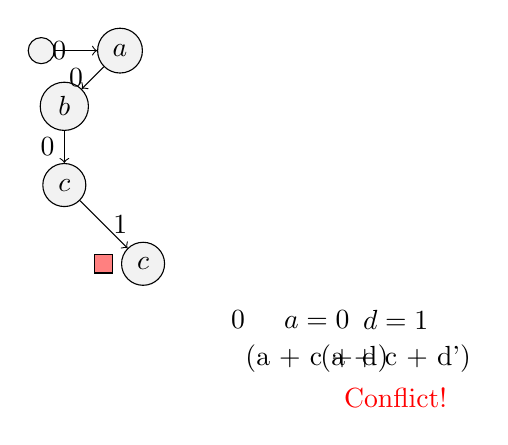
\begin{tikzpicture}[node distance=1cm]
    \node[circle, draw, fill=lightgray!20] (root) {};
    \node[circle, draw, fill=lightgray!20, right of=root] (a) {$a$};
    \node[circle, draw, fill=lightgray!20, below left of=a] (b) {$b$};
    \node[circle, draw, fill=lightgray!20, below of=b] (c) {$c$};
    \draw[->] (root) -- (a) node[midway, left] {0};
    \draw[->] (a) -- (b) node[midway, left] {0};
    \draw[->] (b) -- (c) node[midway, left] {0};
    \node[circle, draw, fill=lightgray!20, below of=c, xshift=1cm] (c1) {$c$};
    \draw[->] (c) -- (c1) node[midway, right] {1};
    \node[rectangle, draw, fill=red!50, below of=c, xshift=0.5cm] {};
    \node[below right of=c1, xshift=0.5cm] {0};
    \node[below right of=c1, xshift=1.5cm] {$a=0$};
    \node[below right of=c1, xshift=1.5cm, yshift=-0.5cm] {(a + c + d)};
    \node[below right of=c1, xshift=2.5cm] {$d=1$};
    \node[below right of=c1, xshift=2.5cm, yshift=-0.5cm] {(a + c + d')};
    \node[below right of=c1, xshift=2.5cm, yshift=-1cm, red] {Conflict!};
\end{tikzpicture}
%
\subsection{Description}%
This slide presents a portion of a search tree, likely part of the Davis-Putnam-Logemann-Loveland (DPLL) algorithm, used for solving the satisfiability (SAT) problem in propositional logic.  The slide shows a set of clauses (disjunctions of literals) in a bulleted list above the tree.  The literals are variables (a, b, c, d) and their negations (a', b', c', d').  The tree diagram visually represents the search space explored by the DPLL algorithm.  Nodes in the tree represent variable assignments.  Edges represent the choices made during the search.  The node labeled "c" has a "1" assignment, indicating a decision made by the algorithm.  A red rectangle below the "c" node suggests a conflict or failure to satisfy the clauses at that point in the search.  Below the "c" node, the slide shows the assignments a=0 and d=1, which led to a conflict, indicated by the "Conflict!" label.  The clauses (a + c + d) and (a + c + d') are shown below the conflict, indicating the clauses that caused the conflict.  The context of the course (Artificial Intelligence Basics) suggests that this slide is part of a lecture on SAT solvers and their strategies for finding satisfying assignments to Boolean formulas. The tree diagram is crucial for understanding the backtracking nature of the DPLL algorithm and how it explores different possibilities to find a solution.%
\subsection{Figures}%
\begin{figure}[H]%
\centering%
\begin{subfigure}[b]{0.15\textwidth}%
\centering%

\includegraphics[width=\textwidth]{/Users/ashoksaravanan/Coding/ScribeLec/server/output/CS 243/lectures/15L2-SAT/figures/28.1.png}%
\caption{}%
\end{subfigure}%
\hspace{0.05\textwidth}%
\begin{subfigure}[b]{0.15\textwidth}%
\centering%

\includegraphics[width=\textwidth]{/Users/ashoksaravanan/Coding/ScribeLec/server/output/CS 243/lectures/15L2-SAT/figures/28.2.png}%
\caption{}%
\end{subfigure}%
\hspace{0.05\textwidth}%
\begin{subfigure}[b]{0.15\textwidth}%
\centering%

\includegraphics[width=\textwidth]{/Users/ashoksaravanan/Coding/ScribeLec/server/output/CS 243/lectures/15L2-SAT/figures/28.3.png}%
\caption{}%
\end{subfigure}%
\end{figure}

%
\newpage%
\section{Slide 29}%
\label{sec:Slide29}%
\subsection{Content}%

\textbf{DPLL Search}

\begin{itemize}
    \item (a' + b + c)
    \item (a + c + d)
    \item (a + c + d')
    \item (a + c' + d)
    \item (a + c' + d')
    \item (b' + c' + d)
    \item (a' + b + c')
    \item (a' + b' + c)
\end{itemize}

\begin{tikzpicture}[node distance=1cm]
    \node[circle, draw, fill=lightgray!20] (root) {};
    \node[circle, draw, fill=lightgray!20, right of=root] (a) {$a$};
    \node[circle, draw, fill=lightgray!20, below left of=a] (b) {$b$};
    \node[circle, draw, fill=lightgray!20, below of=b] (c) {$c$};
    \draw[->] (root) -- (a) node[midway, left] {0};
    \draw[->] (a) -- (b) node[midway, left] {0};
    \draw[->] (b) -- (c) node[midway, left] {0};
    \draw[->, blue] (c) -- node[midway, right] {1 $\leftarrow$ Forced Decision} (c1);
    \node[circle, draw, fill=lightgray!20, below of=c1] (c0) {$c$};
    \draw[->] (c1) -- (c0) node[midway, right] {0};
    \node[rectangle, draw, fill=red!50, below of=c0, xshift=0.5cm] {};
    \node[below right of=c0, xshift=0.5cm] {0};
    \node[below right of=c0, xshift=1.5cm] {$a=0$};
    \node[below right of=c0, xshift=1.5cm, yshift=-0.5cm] {(a + c + d)};
    \node[below right of=c0, xshift=2.5cm] {$d=1$};
    \node[below right of=c0, xshift=2.5cm, yshift=-0.5cm] {(a + c + d')};
    \node[below right of=c0, xshift=2.5cm, yshift=-1cm, red] {Conflict!};
\end{tikzpicture}
%
\subsection{Description}%
This slide presents a portion of a search tree, likely part of the DPLL (Davis-Putnam-Logemann-Loveland) algorithm, used for solving the satisfiability (SAT) problem in propositional logic.  The problem is represented by a set of clauses (disjunctions of literals) in a bulleted list above the tree.  The literals are variables (a, b, c, d) and their negations (a', b', c', d').  The tree diagram visually represents the search space explored by the DPLL algorithm.  Nodes in the tree represent variable assignments.  Edges represent the choices made during the search.  The node labeled "c" has a "1 ← Forced Decision" label, indicating a forced decision for variable c.  A red rectangle below the "c" node indicates a conflict or failure to satisfy the clauses at that point in the search.  Below the "c" node, the slide shows the assignments a=0 and d=1, which led to a conflict, indicated by the "Conflict!" label.  The clauses (a + c + d) and (a + c + d') are shown below the conflict, indicating the clauses that caused the conflict.  The context of the course (Artificial Intelligence Basics) suggests that this slide is part of a lecture on SAT solvers and their strategies for finding satisfying assignments to Boolean formulas. The tree diagram is crucial for understanding the backtracking nature of the DPLL algorithm and how it explores different possibilities to find a solution.%
\subsection{Figures}%
\begin{figure}[H]%
\centering%
\begin{subfigure}[b]{0.15\textwidth}%
\centering%

\includegraphics[width=\textwidth]{/Users/ashoksaravanan/Coding/ScribeLec/server/output/CS 243/lectures/15L2-SAT/figures/29.1.png}%
\caption{}%
\end{subfigure}%
\hspace{0.05\textwidth}%
\begin{subfigure}[b]{0.15\textwidth}%
\centering%

\includegraphics[width=\textwidth]{/Users/ashoksaravanan/Coding/ScribeLec/server/output/CS 243/lectures/15L2-SAT/figures/29.2.png}%
\caption{}%
\end{subfigure}%
\hspace{0.05\textwidth}%
\begin{subfigure}[b]{0.15\textwidth}%
\centering%

\includegraphics[width=\textwidth]{/Users/ashoksaravanan/Coding/ScribeLec/server/output/CS 243/lectures/15L2-SAT/figures/29.3.png}%
\caption{}%
\end{subfigure}%
\end{figure}

%
\newpage%
\section{Slide 30}%
\label{sec:Slide30}%
\subsection{Content}%
%
\subsection{Description}%
This slide, titled "DPLL Search," presents a portion of a search tree for the satisfiability (SAT) problem in the context of Artificial Intelligence Basics. The problem is represented by a set of clauses (disjunctions of literals) in propositional logic. The literals are variables (a, b, c, d) and their negations (a', b', c', d'). The clauses are listed in a bulleted list above the tree. The tree diagram visually represents the search space explored by the DPLL algorithm. The nodes in the tree represent variable assignments. The edges represent the choices made during the search.  The node labeled "a" has an arrow pointing to the right with the label "Backtrack," indicating that the search backtracked from this node.  The nodes labeled "c" and "c1" have assignments of 0 and 1 respectively.  Below these nodes are four red rectangles, suggesting that the assignments at these nodes led to conflicts or failures to satisfy the clauses. The context of the course (Artificial Intelligence Basics) suggests that this slide is part of a lecture on SAT solvers and their strategies for finding satisfying assignments to Boolean formulas. The tree diagram is crucial for understanding the backtracking nature of the DPLL algorithm and how it explores different possibilities to find a solution. The numbers 0 and 1 next to the nodes represent the assigned values to the variables.%
\subsection{Figures}%
\begin{figure}[H]%
\centering%
\begin{subfigure}[b]{0.15\textwidth}%
\centering%

\includegraphics[width=\textwidth]{/Users/ashoksaravanan/Coding/ScribeLec/server/output/CS 243/lectures/15L2-SAT/figures/30.1.png}%
\caption{}%
\end{subfigure}%
\hspace{0.05\textwidth}%
\begin{subfigure}[b]{0.15\textwidth}%
\centering%

\includegraphics[width=\textwidth]{/Users/ashoksaravanan/Coding/ScribeLec/server/output/CS 243/lectures/15L2-SAT/figures/30.2.png}%
\caption{}%
\end{subfigure}%
\hspace{0.05\textwidth}%
\begin{subfigure}[b]{0.15\textwidth}%
\centering%

\includegraphics[width=\textwidth]{/Users/ashoksaravanan/Coding/ScribeLec/server/output/CS 243/lectures/15L2-SAT/figures/30.3.png}%
\caption{}%
\end{subfigure}%
\hspace{0.05\textwidth}%
\begin{subfigure}[b]{0.15\textwidth}%
\centering%

\includegraphics[width=\textwidth]{/Users/ashoksaravanan/Coding/ScribeLec/server/output/CS 243/lectures/15L2-SAT/figures/30.4.png}%
\caption{}%
\end{subfigure}%
\end{figure}

%
\newpage%
\section{Slide 31}%
\label{sec:Slide31}%
\subsection{Content}%

\textbf{DPLL Search}

\begin{itemize}
    \item (a' + b + c)
    \item (a + c + d)
    \item (a + c + d')
    \item (a + c' + d)
    \item (a + c' + d')
    \item (b' + c' + d)
    \item (a' + b + c')
    \item (a' + b' + c)
    \item (a + b + c)
\end{itemize}

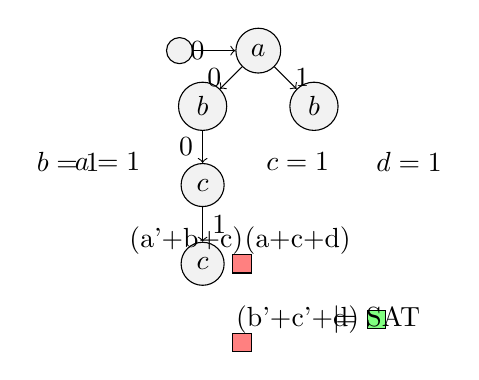
\begin{tikzpicture}[node distance=1cm]
    \node[circle, draw, fill=lightgray!20] (root) {};
    \node[circle, draw, fill=lightgray!20, right of=root] (a) {$a$};
    \node[circle, draw, fill=lightgray!20, below left of=a] (b) {$b$};
    \node[circle, draw, fill=lightgray!20, below of=b] (c) {$c$};
    \node[circle, draw, fill=lightgray!20, below right of=a] (b1) {$b$};
    \node[circle, draw, fill=lightgray!20, below of=c] (c1) {$c$};
    \draw[->] (root) -- (a) node[midway, left] {0};
    \draw[->] (a) -- (b) node[midway, left] {0};
    \draw[->] (b) -- (c) node[midway, left] {0};
    \draw[->] (a) -- (b1) node[midway, right] {1};
    \draw[->] (c) -- (c1) node[midway, right] {1};
    \node[rectangle, draw, fill=red!50, below of=c, xshift=0.5cm] {};
    \node[rectangle, draw, fill=red!50, below of=c1, xshift=0.5cm] {};
    \node[rectangle, draw, fill=green!50, below right of=c1, xshift=1.5cm] {};
    \node[below right of=c1, xshift=1.5cm] {$\models$ SAT};
    \node[below left of=c, xshift=0.5cm] {(a'+b+c)};
    \node[below right of=c, xshift=0.5cm] {(a+c+d)};
    \node[below right of=c1, xshift=0.5cm] {(b'+c'+d)};
    \node[below left of=b, xshift=-0.5cm] {$a=1$};
    \node[below right of=b, xshift=0.5cm] {$c=1$};
    \node[below right of=b1, xshift=0.5cm] {$d=1$};
    \node[below left of=b, xshift=-1cm] {$b=1$};
\end{tikzpicture}
%
\subsection{Description}%
This slide presents a DPLL (Davis-Putnam-Logemann-Loveland) search tree for a propositional logic problem. The problem is represented by a set of clauses (disjunctions of literals) in the bulleted list above the tree. The literals are variables (a, b, c, d) and their negations (a', b', c', d'). The tree visually depicts the search space explored by the DPLL algorithm.  Nodes in the tree represent variable assignments. Edges represent the choices made during the search.  The slide shows a complete search path that leads to a satisfying assignment, indicated by the green rectangle labeled "$\models$ SAT" at the bottom right of the tree.  The assignments $a=1$, $b=1$, $c=1$, and $d=1$ are shown below the tree, indicating the values that satisfy all the clauses. The context of the course (Artificial Intelligence Basics) suggests that this slide is part of a lecture on SAT solvers and their strategies for finding satisfying assignments to Boolean formulas. The tree diagram is crucial for understanding the backtracking nature of the DPLL algorithm and how it explores different possibilities to find a solution.%
\subsection{Figures}%
\begin{figure}[H]%
\centering%
\begin{subfigure}[b]{0.15\textwidth}%
\centering%

\includegraphics[width=\textwidth]{/Users/ashoksaravanan/Coding/ScribeLec/server/output/CS 243/lectures/15L2-SAT/figures/31.1.png}%
\caption{}%
\end{subfigure}%
\hspace{0.05\textwidth}%
\begin{subfigure}[b]{0.15\textwidth}%
\centering%

\includegraphics[width=\textwidth]{/Users/ashoksaravanan/Coding/ScribeLec/server/output/CS 243/lectures/15L2-SAT/figures/31.2.png}%
\caption{}%
\end{subfigure}%
\hspace{0.05\textwidth}%
\begin{subfigure}[b]{0.15\textwidth}%
\centering%

\includegraphics[width=\textwidth]{/Users/ashoksaravanan/Coding/ScribeLec/server/output/CS 243/lectures/15L2-SAT/figures/31.3.png}%
\caption{}%
\end{subfigure}%
\hspace{0.05\textwidth}%
\begin{subfigure}[b]{0.15\textwidth}%
\centering%

\includegraphics[width=\textwidth]{/Users/ashoksaravanan/Coding/ScribeLec/server/output/CS 243/lectures/15L2-SAT/figures/31.4.png}%
\caption{}%
\end{subfigure}%
\hspace{0.05\textwidth}%
\begin{subfigure}[b]{0.15\textwidth}%
\centering%

\includegraphics[width=\textwidth]{/Users/ashoksaravanan/Coding/ScribeLec/server/output/CS 243/lectures/15L2-SAT/figures/31.5.png}%
\caption{}%
\end{subfigure}%
\end{figure}

%
\newpage%
\section{Slide 32}%
\label{sec:Slide32}%
\subsection{Content}%

\textbf{Resolution Rule}

If a formula $\phi$ contains clauses $(x \vee \alpha)$ and $(\neg x \vee \beta)$,
then one can derive a new clause $(\alpha \vee \beta)$
%
\subsection{Description}%
This slide presents the Resolution Rule in propositional logic.  It states that if a formula $\phi$ contains two clauses, one containing a literal $x$ and the other containing the negation of that literal $\neg x$, then a new clause can be derived by combining the remaining literals from each clause.  In this case, the new clause is formed by combining $\alpha$ and $\beta$, resulting in the clause $(\alpha \vee \beta)$. The context of the course (Artificial Intelligence Basics) suggests that this slide is part of a lecture on automated theorem proving and specifically on the resolution method for proving logical statements.  The resolution rule is a key inference rule in resolution-based theorem provers.%
\subsection{Figures}%
\begin{figure}[H]%
\centering%
\end{figure}

%
\newpage%
\section{Slide 33}%
\label{sec:Slide33}%
\subsection{Content}%

\textbf{What clauses can resolution be applied?}

\begin{itemize}
    \item (a' + b + c)
    \item (a + c + d)
    \item (a + c + d')
    \item (a + c' + d)
    \item (a + c' + d')
    \item (b' + c' + d)
    \item (a' + b + c')
    \item (a' + b' + c)
    \item (a + b + c)
\end{itemize}

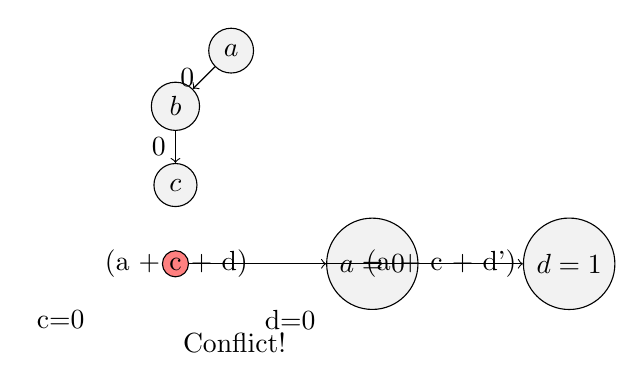
\begin{tikzpicture}[node distance=1cm]
    \node[circle, draw, fill=lightgray!20] (a) {$a$};
    \node[circle, draw, fill=lightgray!20, below left of=a] (b) {$b$};
    \node[circle, draw, fill=lightgray!20, below of=b] (c) {$c$};
    \node[circle, draw, fill=red!50, below of=c] (conflict) {};
    \node[circle, draw, fill=lightgray!20, right of=conflict, xshift=1.5cm] (a_eq_0) {$a=0$};
    \node[circle, draw, fill=lightgray!20, right of=a_eq_0, xshift=1.5cm] (d_eq_1) {$d=1$};
    \draw[->] (a) -- (b) node[midway, left] {0};
    \draw[->] (b) -- (c) node[midway, left] {0};
    \draw[->] (conflict) -- (a_eq_0) node[midway, left] {(a + c + d)};
    \draw[->] (conflict) -- (d_eq_1) node[midway, right] {(a + c + d')};
    \node[below of=conflict, xshift=0.75cm] {Conflict!};
    \node[below left of=conflict, xshift=-0.75cm] {c=0};
    \node[below right of=conflict, xshift=0.75cm] {d=0};
\end{tikzpicture}

\end{tikzpicture}
%
\subsection{Description}%
This slide, titled "What clauses can resolution be applied?", presents a set of clauses (disjunctions of literals) in propositional logic.  The literals are variables (a, b, c, d) and their negations (a', b', c', d').  The clauses are listed in a bulleted list above a visual representation of an implication graph.  The implication graph shows a search tree-like structure where nodes represent variable assignments.  The nodes are labeled with the variable and its assigned value (0 or 1).  Arrows indicate the order of assignments.  A red box/rectangle below the node 'c' indicates a conflict.  The slide highlights the application of the unit propagation method, which quickly determines conflicts in the search space.  The implication graph shows that assigning a=0 and d=1 leads to a conflict, as indicated by the red box/rectangle.  The clauses (a + c + d) and (a + c + d') are shown as connected to the conflict node, indicating that these clauses are involved in the conflict.  The context of the course (Artificial Intelligence Basics) suggests that this slide is part of a lecture on SAT solvers and their strategies for finding satisfying assignments to Boolean formulas. The implication graph is crucial for understanding how the algorithm explores different possibilities to find a solution and how unit propagation helps to identify conflicts early in the search process.%
\subsection{Figures}%
\begin{figure}[H]%
\centering%
\begin{subfigure}[b]{0.15\textwidth}%
\centering%

\includegraphics[width=\textwidth]{/Users/ashoksaravanan/Coding/ScribeLec/server/output/CS 243/lectures/15L2-SAT/figures/33.1.png}%
\caption{}%
\end{subfigure}%
\hspace{0.05\textwidth}%
\begin{subfigure}[b]{0.15\textwidth}%
\centering%

\includegraphics[width=\textwidth]{/Users/ashoksaravanan/Coding/ScribeLec/server/output/CS 243/lectures/15L2-SAT/figures/33.2.png}%
\caption{}%
\end{subfigure}%
\end{figure}

%
\newpage%
\section{Slide 34}%
\label{sec:Slide34}%
\subsection{Content}%

\textbf{Clause Learning}

\begin{itemize}
    \item (a' + b + c)
    \item (a + c + d)
    \item (a + c + d')
    \item (a + c' + d)
    \item (a + c' + d')
    \item (b' + c' + d)
    \item (a' + b + c')
    \item (a' + b' + c)
    \item (a + b + c)
\end{itemize}

\begin{tikzpicture}[node distance=1cm]
    \node[circle, draw, fill=lightgray!20] (a) {$a$};
    \node[circle, draw, fill=lightgray!20, below left of=a] (b) {$b$};
    \node[circle, draw, fill=lightgray!20, below of=b] (c) {$c$};
    \node[circle, draw, fill=red!50, below of=c] (conflict) {};
    \node[circle, draw, fill=lightgray!20, right of=conflict, xshift=1.5cm, yshift=-0.5cm] (a_eq_0) {$a=0$};
    \node[circle, draw, fill=lightgray!20, right of=a_eq_0, xshift=1.5cm, yshift=-0.5cm] (d_eq_1) {$d=1$};
    \draw[->] (a) -- (b) node[midway, left] {0};
    \draw[->] (b) -- (c) node[midway, left] {0};
    \draw[->] (conflict) -- (a_eq_0) node[midway, left] {(a + c + d)};
    \draw[->] (conflict) -- (d_eq_1) node[midway, right] {(a + c + d')};
    \node[below of=conflict, xshift=0.75cm] {Conflict!};
    \node[below left of=conflict, xshift=-0.75cm] {c=0};
    \node[below right of=conflict, xshift=0.75cm] {d=0};
    \node[below right of=conflict, xshift=2.5cm, yshift=-1cm] {¬a∨¬c};
\end{tikzpicture}

\end{tikzpicture}
%
\subsection{Description}%
This slide, titled "Clause Learning," presents a set of clauses (disjunctions of literals) in propositional logic. The literals are variables (a, b, c, d) and their negations (a', b', c', d'). The clauses are listed in a bulleted list above a visual representation of an implication graph. The implication graph shows a search tree-like structure where nodes represent variable assignments.  Nodes are labeled with the variable and its assigned value (0 or 1). Arrows indicate the order of assignments. A red box/rectangle below the node 'c' indicates a conflict. The slide highlights the application of the unit propagation method, which quickly determines conflicts in the search space. The implication graph shows that assigning a=0 and d=1 leads to a conflict, as indicated by the red box/rectangle. The clauses (a + c + d) and (a + c + d') are shown as connected to the conflict node, indicating that these clauses are involved in the conflict.  The new clause ¬a∨¬c is shown below the conflict node, indicating that this clause has been learned from the conflict. The context of the course (Artificial Intelligence Basics) suggests that this slide is part of a lecture on SAT solvers and their strategies for finding satisfying assignments to Boolean formulas. The implication graph is crucial for understanding how the algorithm explores different possibilities to find a solution and how unit propagation helps to identify conflicts early in the search process. The new clause ¬a∨¬c is added to the original clause database to avoid revisiting the same conflict in future searches.%
\subsection{Figures}%
\begin{figure}[H]%
\centering%
\begin{subfigure}[b]{0.15\textwidth}%
\centering%

\includegraphics[width=\textwidth]{/Users/ashoksaravanan/Coding/ScribeLec/server/output/CS 243/lectures/15L2-SAT/figures/34.1.png}%
\caption{}%
\end{subfigure}%
\hspace{0.05\textwidth}%
\begin{subfigure}[b]{0.15\textwidth}%
\centering%

\includegraphics[width=\textwidth]{/Users/ashoksaravanan/Coding/ScribeLec/server/output/CS 243/lectures/15L2-SAT/figures/34.2.png}%
\caption{}%
\end{subfigure}%
\end{figure}

%
\newpage%
\section{Slide 35}%
\label{sec:Slide35}%
\subsection{Content}%

\textbf{Key Advances in SAT Reasoning}

\begin{itemize}
    \item Learn from mistakes during search
    \item Never make similar mistakes again!!
    \item Clause Learning: when DPLL backtracks,
    learn a concise reason: what went wrong
    \item → avoid similar ‘mistakes’ in the future!
    \item Extremely powerful in practice
    \item Restart to avoid heavy-tailed behavior
    \item Trade-off between “refine on what we have” vs. “exploring something new”
    \item SAT solvers known to sometimes “get stuck” and at other times be very fast… on similar problems, of similar size, etc.
    \item Discovery: runtime distribution (across ‘similar’ instances or even on a single instance) is heavy-tailed $\implies$ too many runs that can take way longer than the average!
    \item Solution: restart computation differently, keep learned clauses!
\end{itemize}

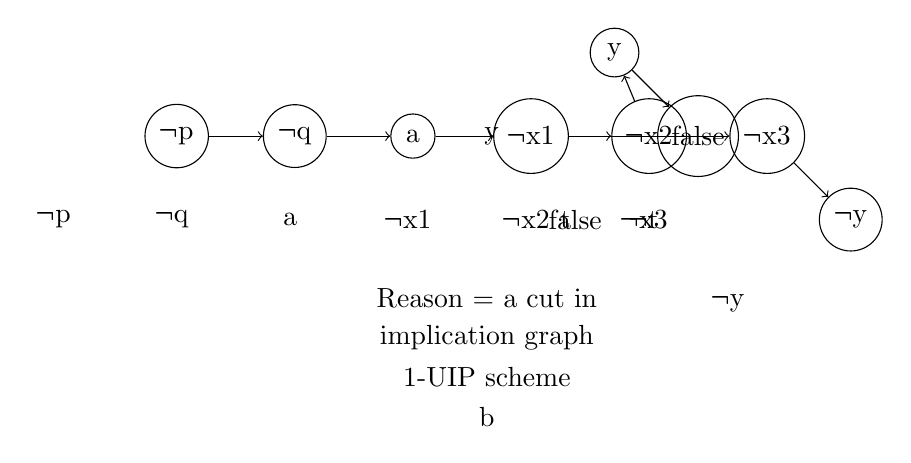
\begin{tikzpicture}[node distance=1.5cm]
    \node[draw, circle] (p) {¬p};
    \node[draw, circle, right of=p] (q) {¬q};
    \node[draw, circle, right of=q] (a) {a};
    \node[draw, circle, right of=a] (x1) {¬x1};
    \node[draw, circle, right of=x1] (x2) {¬x2};
    \node[draw, circle, right of=x2] (x3) {¬x3};
    \node[draw, circle, above right of=x1] (y) {y};
    \node[draw, circle, below right of=x3] (ny) {¬y};
    \node[draw, circle, below right of=y] (false) {false};
    \draw[->] (p) -- (q);
    \draw[->] (q) -- (a);
    \draw[->] (a) -- (x1);
    \draw[->] (x1) -- (x2);
    \draw[->] (x1) -- (x3);
    \draw[->] (x2) -- (y);
    \draw[->] (x3) -- (ny);
    \draw[->] (y) -- (false);
    \node[below left of=p, xshift=-0.5cm] {¬p};
    \node[below left of=q, xshift=-0.5cm] {¬q};
    \node[below left of=a, xshift=-0.5cm] {a};
    \node[below left of=x1, xshift=-0.5cm] {¬x1};
    \node[below left of=x2, xshift=-0.5cm] {¬x2};
    \node[below left of=x3, xshift=-0.5cm] {¬x3};
    \node[below left of=y, xshift=-0.5cm] {y};
    \node[below left of=ny, xshift=-0.5cm] {¬y};
    \node[below left of=false, xshift=-0.5cm] {false};
    \node[below left of=x1, xshift=1.5cm] {t};
    \node[below left of=x1, xshift=2.5cm] {¬t};
    \node[below left of=x1, xshift=0.5cm, yshift=-1cm] {Reason = a cut in};
    \node[below left of=x1, xshift=0.5cm, yshift=-1.5cm] {implication graph};
    \node[below left of=x1, xshift=0.5cm, yshift=-2cm] {1-UIP scheme};
    \node[below left of=x1, xshift=0.5cm, yshift=-2.5cm] {b};
\end{tikzpicture}
%
\subsection{Description}%
This slide, titled "Key Advances in SAT Reasoning," summarizes key improvements in SAT (Satisfiability) solvers.  It discusses techniques for learning from mistakes during the search process, specifically highlighting "Clause Learning."  Clause Learning is described as a method used when a DPLL (Davis-Putnam-Logemann-Loveland) backtracking algorithm fails.  In this case, the solver learns a concise reason for the failure and avoids making the same mistake in the future.  The slide also emphasizes the importance of restarts to avoid "heavy-tailed" behavior in SAT solvers.  Heavy-tailed behavior refers to the runtime distribution of SAT solvers, where some instances take significantly longer than average to solve.  The slide suggests that a trade-off exists between refining existing strategies and exploring new ones.  The slide also mentions the discovery that SAT solver runtime distributions are often heavy-tailed, meaning that some instances take much longer than average to solve.  The solution proposed is to restart the computation differently and to keep learned clauses.  The accompanying diagram illustrates a portion of an implication graph, a crucial data structure in SAT solvers.  The graph shows the relationships between literals (variables and their negations) and their implications.  The context of the course (Artificial Intelligence Basics) suggests that this slide is part of a lecture on automated theorem proving and specifically on the resolution method for proving logical statements.  The diagram is a visual representation of the implication graph, which is used to determine the satisfiability of a Boolean formula.%
\subsection{Figures}%
\begin{figure}[H]%
\centering%
\end{figure}

%
\newpage%
\section{Slide 36}%
\label{sec:Slide36}%
\subsection{Content}%

\textbf{Key Advances in SAT Reasoning}

\begin{itemize}
    \item Machine learning to build algorithm portfolios
    \item Observation: no single SAT solver is good on every family of instances
    \item Features of a given instance can be used to predict, with reasonable accuracy, which solver will work well on it!
    \item Solution: design a portfolio solver using ML techniques
    \item Based on runtime prediction models
    \item Recent work - avoid complex models, use k-NN or clustering
    \item Automatic parameter tuning (generic and instance-specific)
    \item SAT solvers are designed with many 'hardwired' parameters
    \item Millions of parameter combinations - impossible to explore all by hand!
    \item Solution: use automatic parameter tuning tools based on local search, genetic algorithms, etc.
    \item Efficient unit propagation
    \item Data structures: watch-out tables (Chaff); Bitwise operation; Cache strategy, etc.
\end{itemize}
%
\subsection{Description}%
This slide, titled "Key Advances in SAT Reasoning," details advancements in SAT solvers.  It emphasizes the use of machine learning to create portfolios of solvers, recognizing that no single solver is universally effective.  The slide highlights the ability to predict which solver will perform best on a given instance based on its features.  The solution involves designing a portfolio solver using machine learning techniques, focusing on runtime prediction models.  Recent work is mentioned, suggesting a shift towards simpler models like k-NN or clustering for prediction.  The slide also discusses automatic parameter tuning, a crucial aspect of SAT solver optimization.  SAT solvers often have many configurable parameters, and the sheer number of possible combinations makes manual tuning impractical.  Therefore, automatic tuning tools based on local search or genetic algorithms are presented as solutions.  Finally, the slide touches upon efficient unit propagation and the use of advanced data structures like watch-out tables (Chaff), bitwise operations, and caching strategies, all contributing to the performance of modern SAT solvers.  The context of the course (Artificial Intelligence Basics) places this slide within a discussion of automated reasoning and problem-solving techniques, specifically focusing on the efficiency and effectiveness of SAT solvers.%
\subsection{Figures}%
\begin{figure}[H]%
\centering%
\end{figure}

%
\newpage%
\section{Slide 37}%
\label{sec:Slide37}%
\subsection{Content}%

\textbf{Solving Real-world problems using SAT}
%
\subsection{Description}%
This slide, likely a title slide or introductory slide for a section on SAT (Satisfiability) solvers in a course on Artificial Intelligence Basics, simply states the topic: "Solving Real-world problems using SAT".  No further details are provided on the slide itself.%
\subsection{Figures}%
\begin{figure}[H]%
\centering%
\end{figure}

%
\newpage%
\section{Slide 38}%
\label{sec:Slide38}%
\subsection{Content}%

\textbf{General Automated Reasoning}

Research Objective: Better reasoning and modeling technology

\begin{itemize}
    \item Problem Instance
    \item Domain Specific
        \begin{itemize}
            \item e.g., logistics, chess, planning, verification, ...
        \end{itemize}
    \item Model Generator (Encoder)
        \begin{itemize}
            \item Generic
            \item Applicable to all domains within range of modeling language
        \end{itemize}
    \item General Inference Engine
    \item Solution
\end{itemize}

Impact: Faster solutions in several domains
\end{itemize}
%
\subsection{Description}%
This slide, likely part of a presentation on AI, discusses a research objective focused on general automated reasoning.  It outlines a process for achieving better reasoning and modeling technology.  The process involves a Problem Instance, which is then processed by a Domain Specific Model Generator (Encoder).  This step is followed by a Generic Model Generator (Encoder) that is applicable to all domains within the range of the modeling language.  The output of the Generic Model Generator is then processed by a General Inference Engine, which produces a Solution.  The slide uses a flowchart-like structure to illustrate the steps involved.  The examples of Domain Specific problems include logistics, chess, planning, and verification.  The impact of this approach is stated as faster solutions in several domains.  The context of the course (Artificial Intelligence Basics) suggests that this slide is part of a discussion on automated reasoning techniques and their application to various problem domains.%
\subsection{Figures}%
\begin{figure}[H]%
\centering%
\begin{subfigure}[b]{0.15\textwidth}%
\centering%

\includegraphics[width=\textwidth]{/Users/ashoksaravanan/Coding/ScribeLec/server/output/CS 243/lectures/15L2-SAT/figures/38.1.png}%
\caption{}%
\end{subfigure}%
\hspace{0.05\textwidth}%
\begin{subfigure}[b]{0.15\textwidth}%
\centering%

\includegraphics[width=\textwidth]{/Users/ashoksaravanan/Coding/ScribeLec/server/output/CS 243/lectures/15L2-SAT/figures/38.2.png}%
\caption{}%
\end{subfigure}%
\hspace{0.05\textwidth}%
\begin{subfigure}[b]{0.15\textwidth}%
\centering%

\includegraphics[width=\textwidth]{/Users/ashoksaravanan/Coding/ScribeLec/server/output/CS 243/lectures/15L2-SAT/figures/38.3.png}%
\caption{}%
\end{subfigure}%
\hspace{0.05\textwidth}%
\begin{subfigure}[b]{0.15\textwidth}%
\centering%

\includegraphics[width=\textwidth]{/Users/ashoksaravanan/Coding/ScribeLec/server/output/CS 243/lectures/15L2-SAT/figures/38.4.png}%
\caption{}%
\end{subfigure}%
\end{figure}

%
\newpage%
\section{Slide 39}%
\label{sec:Slide39}%
\subsection{Content}%

\textbf{The Challenge of Exponential Complexity Growth}

\textit{Note:} rough estimates, for propositional reasoning

\begin{tikzpicture}
\begin{axis}[
    title={Exponential Complexity Growth},
    xlabel={Exponential Complexity},
    ylabel={Case complexity},
    xmin=0, xmax=1000000,
    ymin=0, ymax=1000000000000000000,
    log basis x=10,
    log basis y=10,
    xtick={100, 1000, 10000, 100000, 1000000},
    ytick={10^0, 10^3, 10^4, 10^7, 10^10, 10^15, 10^20},
    legend pos=south east,
    ymajorgrids=true,
    xmajorgrids=true,
]

\addplot[domain=1:1000000, samples=100, color=blue, thick] {x};
\addlegendentry{Exponential Complexity};

\addplot[only marks, mark=*, mark size=2pt, color=red] coordinates {
(100, 10^3)
(1000, 10^4)
(10000, 10^7)
(100000, 10^10)
(1000000, 10^15)
};
\addlegendentry{Case Complexity};

\node[anchor=north west] at (axis cs:100, 10^3) {100};
\node[anchor=north west] at (axis cs:1000, 10^4) {10K};
\node[anchor=north west] at (axis cs:10000, 10^7) {100K};
\node[anchor=north west] at (axis cs:100000, 10^10) {1M};
\node[anchor=north west] at (axis cs:1000000, 10^15) {10^15};

\node[anchor=south west] at (axis cs:100, 10^3) {Car repair diagnosis};
\node[anchor=south west] at (axis cs:1000, 10^4) {Deep space mission control};
\node[anchor=south west] at (axis cs:10000, 10^7) {Chess (20 steps deep)};
\node[anchor=south west] at (axis cs:100000, 10^10) {Military Logistics};
\node[anchor=south west] at (axis cs:1000000, 10^15) {VLSI Verification};
\node[anchor=south west] at (axis cs:1000000, 10^15) {War Gaming};

\node[anchor=north west] at (axis cs:100, 10^3) {100};
\node[anchor=north west] at (axis cs:1000, 10^4) {10K};
\node[anchor=north west] at (axis cs:10000, 10^7) {100K};
\node[anchor=north west] at (axis cs:100000, 10^10) {1M};
\node[anchor=north west] at (axis cs:1000000, 10^15) {10^15};

\end{axis}
\end{tikzpicture}

\begin{itemize}
    \item No. of atoms on the earth ($10^{30}$)
    \item Seconds until heat death of sun ($10^{47}$)
    \item Protein folding calculation (petaflop-year) ($10^{30}$)
\end{itemize}

\textit{Credit:} Kumar, DARPA; cited in Computer World magazine

\end{itemize}
%
\subsection{Description}%
This slide, titled "The Challenge of Exponential Complexity Growth," presents a graph illustrating the exponential growth of computational complexity in various real-world problems.  The x-axis represents the number of variables or rules (logarithmic scale), and the y-axis represents the computational complexity (logarithmic scale).  The graph shows a steep upward trend, indicating that the computational resources required to solve problems increase exponentially as the problem size grows.  The slide highlights several examples of problems with varying complexities, including car repair diagnosis (100 variables), deep space mission control (10K variables), chess (20 steps deep, 100K variables), military logistics (100K variables), VLSI verification (1M variables), and war gaming (1M variables).  The slide also includes examples of real-world phenomena with corresponding computational complexities, such as the number of atoms on Earth ($10^{30}$), the time until the heat death of the sun ($10^{47}$), and protein folding calculations (petaflop-year, $10^{30}$).  The context of the course (Artificial Intelligence Basics) suggests that this slide is part of a discussion on the limitations of computational resources when dealing with complex problems, particularly in the context of propositional reasoning.%
\subsection{Figures}%
\begin{figure}[H]%
\centering%
\begin{subfigure}[b]{0.15\textwidth}%
\centering%

\includegraphics[width=\textwidth]{/Users/ashoksaravanan/Coding/ScribeLec/server/output/CS 243/lectures/15L2-SAT/figures/39.1.png}%
\caption{}%
\end{subfigure}%
\hspace{0.05\textwidth}%
\begin{subfigure}[b]{0.15\textwidth}%
\centering%

\includegraphics[width=\textwidth]{/Users/ashoksaravanan/Coding/ScribeLec/server/output/CS 243/lectures/15L2-SAT/figures/39.2.png}%
\caption{}%
\end{subfigure}%
\hspace{0.05\textwidth}%
\begin{subfigure}[b]{0.15\textwidth}%
\centering%

\includegraphics[width=\textwidth]{/Users/ashoksaravanan/Coding/ScribeLec/server/output/CS 243/lectures/15L2-SAT/figures/39.3.png}%
\caption{}%
\end{subfigure}%
\hspace{0.05\textwidth}%
\begin{subfigure}[b]{0.15\textwidth}%
\centering%

\includegraphics[width=\textwidth]{/Users/ashoksaravanan/Coding/ScribeLec/server/output/CS 243/lectures/15L2-SAT/figures/39.4.png}%
\caption{}%
\end{subfigure}%
\hspace{0.05\textwidth}%
\begin{subfigure}[b]{0.15\textwidth}%
\centering%

\includegraphics[width=\textwidth]{/Users/ashoksaravanan/Coding/ScribeLec/server/output/CS 243/lectures/15L2-SAT/figures/39.5.png}%
\caption{}%
\end{subfigure}%
\end{figure}

%
\newpage%
\section{Slide 40}%
\label{sec:Slide40}%
\subsection{Content}%
%
\subsection{Description}%
This slide, part of a lecture on Artificial Intelligence Basics, introduces the problem of encoding a Hamiltonian Path Problem into a Satisfiability (SAT) problem.  It defines the Hamiltonian Path Problem as finding a path in a directed graph that visits each vertex exactly once.  The slide shows a directed graph with vertices labeled 1 through 5, and edges connecting them.  The question posed is whether a Hamiltonian path exists in this specific graph.  The slide also includes the sequence $1 \rightarrow 3 \rightarrow 4 \rightarrow 2 \rightarrow 5$ as an example of a possible path, and asks how a SAT solver can be used to determine if such a path exists. The context suggests that the slide is part of a discussion on using SAT solvers to solve graph problems in AI.%
\subsection{Figures}%
\begin{figure}[H]%
\centering%
\begin{subfigure}[b]{0.15\textwidth}%
\centering%

\includegraphics[width=\textwidth]{/Users/ashoksaravanan/Coding/ScribeLec/server/output/CS 243/lectures/15L2-SAT/figures/40.1.png}%
\caption{}%
\end{subfigure}%
\end{figure}

%
\newpage%
\section{Slide 41}%
\label{sec:Slide41}%
\subsection{Content}%

\textbf{Encode Hamiltonian Path Problem into SAT}

Hamiltonian Path Problem

\begin{itemize}
    \item Encode the problem into SAT.
    \item Use an off-the-shelf SAT solver to solve the instance.
    \item Convert the assignments of Boolean variables to an actual path.
\end{itemize}

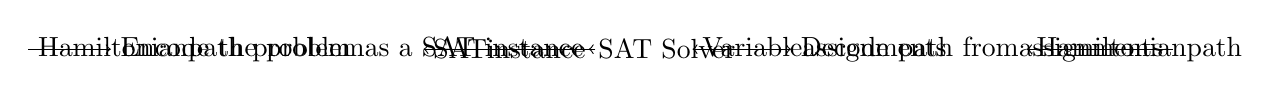
\begin{tikzpicture}[node distance=2cm]
\node (hamiltonian) {Hamiltonian \\ path problem};
\node[right of=hamiltonian] (encode) {Encode the problem \\ as a SAT instance};
\node[right of=encode] (sat_instance) {SAT \\ instance};
\node[right of=sat_instance] (sat_solver) {SAT Solver};
\node[right of=sat_solver] (variable_assignments) {Variable \\ assignments};
\node[right of=variable_assignments] (decode) {Decode path from \\ assignments};
\node[right of=decode] (hamiltonian_path) {Hamiltonian \\ path};

\draw[->] (hamiltonian) -- (encode);
\draw[->] (encode) -- (sat_instance);
\draw[->] (sat_instance) -- (sat_solver);
\draw[->] (sat_solver) -- (variable_assignments);
\draw[->] (variable_assignments) -- (decode);
\draw[->] (decode) -- (hamiltonian_path);
\end{tikzpicture}
\end{latex}
%
\subsection{Description}%
This slide, part of a lecture on Artificial Intelligence Basics, outlines a method for solving the Hamiltonian Path Problem using a Satisfiability (SAT) solver.  The Hamiltonian Path Problem is defined as finding a path in a directed graph that visits each vertex exactly once.  The slide presents a flowchart-like diagram illustrating the process.  The process begins with the Hamiltonian Path Problem.  The problem is then encoded into a Satisfiability (SAT) instance.  This SAT instance is then fed into an off-the-shelf SAT solver.  The SAT solver returns variable assignments.  Finally, these variable assignments are decoded to produce an actual path.  The diagram visually represents the steps involved in the process, showing the flow of information from the initial problem to the final solution.  The context of the course suggests that this slide is part of a discussion on problem encoding and using SAT solvers for graph problems in AI.%
\subsection{Figures}%
\begin{figure}[H]%
\centering%
\begin{subfigure}[b]{0.15\textwidth}%
\centering%

\includegraphics[width=\textwidth]{/Users/ashoksaravanan/Coding/ScribeLec/server/output/CS 243/lectures/15L2-SAT/figures/41.1.png}%
\caption{}%
\end{subfigure}%
\end{figure}

%
\newpage%
\section{Slide 42}%
\label{sec:Slide42}%
\subsection{Content}%

\textbf{Encode Hamiltonian Path Problem into SAT}

\textbf{Variables Design:}

\begin{itemize}
    \item As the path will visit vertices one by one, our propositions should somehow be related to either vertices or edges.
    \item A path consists of a sequence of vertices and edges. Our propositions must also relate to some ordering.
\end{itemize}

Let's propose variables $\{h_{ij}\}$

\begin{itemize}
    \item $h_{ij}$: The $i^{th}$ vertex visited in the path is vertex $j$
    \item Path length = \#Nodes = 5, so $i$ and $j$ both take value from \{1, 2, 3, 4, 5\}
\end{itemize}

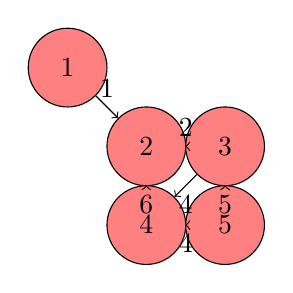
\begin{tikzpicture}
\node[draw, circle, fill=red!50, minimum size=1cm] (1) at (0, 3) {1};
\node[draw, circle, fill=red!50, minimum size=1cm] (2) at (1, 2) {2};
\node[draw, circle, fill=red!50, minimum size=1cm] (3) at (2, 2) {3};
\node[draw, circle, fill=red!50, minimum size=1cm] (4) at (1, 1) {4};
\node[draw, circle, fill=red!50, minimum size=1cm] (5) at (2, 1) {5};

\draw[->] (1) -- (2) node[midway, above] {1};
\draw[->] (2) -- (3) node[midway, above] {2};
\draw[->] (2) -- (4) node[midway, below] {6};
\draw[->] (3) -- (4) node[midway, below] {4};
\draw[->] (3) -- (5) node[midway, below] {5};
\draw[->] (4) -- (5) node[midway, below] {4};
\end{tikzpicture}
\end{latex}
%
\subsection{Description}%
This slide, part of a lecture on Artificial Intelligence Basics, outlines the variable design for encoding the Hamiltonian Path Problem into a Satisfiability (SAT) problem.  The slide introduces the concept of encoding a path through a graph using Boolean variables.  It states that the path will visit vertices one by one, and propositions will relate to either vertices or edges in the graph.  A path is defined as a sequence of vertices and edges, with a specific ordering.  The slide proposes variables $h_{ij}$, where $h_{ij}$ represents the proposition that the $i^{th}$ vertex visited in the path is vertex $j$.  The path length is specified as 5, meaning that $i$ and $j$ both take values from the set {1, 2, 3, 4, 5}.  A directed graph is included, illustrating the vertices and edges of the problem.  The vertices are numbered 1 through 5, and edges connect them.  The numbers on the edges represent weights or constraints.  The context of the slide suggests that this is part of a discussion on using SAT solvers to solve graph problems in AI, specifically the Hamiltonian Path Problem.%
\subsection{Figures}%
\begin{figure}[H]%
\centering%
\begin{subfigure}[b]{0.15\textwidth}%
\centering%

\includegraphics[width=\textwidth]{/Users/ashoksaravanan/Coding/ScribeLec/server/output/CS 243/lectures/15L2-SAT/figures/42.1.png}%
\caption{}%
\end{subfigure}%
\end{figure}

%
\newpage%
\section{Slide 43}%
\label{sec:Slide43}%
\subsection{Content}%

\textbf{Encode Hamiltonian Path Problem into SAT}

Next, consider the constraints when assigning values

\begin{itemize}
    \item Translate: first vertex of the Hamiltonian path cannot be two distinct vertices at the same time
    \item $(h_{11} \implies \neg h_{12}) \land (h_{11} \implies \neg h_{13}) \land (h_{11} \implies \neg h_{14}) \land (h_{11} \implies \neg h_{15}) \land$
    \item $(h_{12} \implies \neg h_{13}) \land (h_{12} \implies \neg h_{14}) \land (h_{12} \implies \neg h_{15}) \land$
    \item $(h_{13} \implies \neg h_{14}) \land (h_{13} \implies \neg h_{15}) \land$
    \item $(h_{14} \implies \neg h_{15})$
\end{itemize}

This is tedious to write but the structure is simple. Let's do it for every vertex of the Hamiltonian path.

Now we can guarantee that at most one node is assigned to a certain place in the Hamiltonian path.

$h_{ij}$: The $i^{th}$ vertex visited in the path is vertex $j$
\end{latex}
%
\subsection{Description}%
This slide, part of a lecture on Artificial Intelligence Basics, details the encoding of the Hamiltonian Path Problem into a Satisfiability (SAT) problem.  It focuses on the constraints required to ensure that only one vertex is visited at each step of the path.  The slide introduces a series of implications, represented using logical connectives (e.g., $\implies$, $\land$).  These implications ensure that if vertex 1 is visited at position $i$, then no other vertex can be visited at position $i$.  The slide explicitly shows the constraints for the first vertex (position 1), demonstrating how these constraints are applied to each vertex in the path.  The notation $h_{ij}$ is defined as the proposition that the $i^{th}$ vertex in the path is vertex $j$.  The context of the slide suggests that this is part of a discussion on using SAT solvers to solve graph problems in AI, specifically the Hamiltonian Path Problem, and how to encode the constraints of the problem into a SAT instance.%
\subsection{Figures}%
\begin{figure}[H]%
\centering%
\begin{subfigure}[b]{0.15\textwidth}%
\centering%

\includegraphics[width=\textwidth]{/Users/ashoksaravanan/Coding/ScribeLec/server/output/CS 243/lectures/15L2-SAT/figures/43.1.png}%
\caption{}%
\end{subfigure}%
\hspace{0.05\textwidth}%
\begin{subfigure}[b]{0.15\textwidth}%
\centering%

\includegraphics[width=\textwidth]{/Users/ashoksaravanan/Coding/ScribeLec/server/output/CS 243/lectures/15L2-SAT/figures/43.2.png}%
\caption{}%
\end{subfigure}%
\hspace{0.05\textwidth}%
\begin{subfigure}[b]{0.15\textwidth}%
\centering%

\includegraphics[width=\textwidth]{/Users/ashoksaravanan/Coding/ScribeLec/server/output/CS 243/lectures/15L2-SAT/figures/43.3.png}%
\caption{}%
\end{subfigure}%
\end{figure}

%
\newpage%
\section{Slide 44}%
\label{sec:Slide44}%
\subsection{Content}%

\textbf{Encode Hamiltonian Path Problem into SAT}

\begin{itemize}
    \item Encode Hamiltonian Path Problem into SAT
    \item Then, enforce selection of exactly one vertex at each step
    \item Firstly, we want to select at least one vertex at the first step,
    \item $(h_{11} \lor h_{12} \lor h_{13} \lor h_{14} \lor h_{15})$
    \item Let's do it for every vertex of the Hamiltonian path!
    \item Now we could guarantee that exactly one node is assigned to a certain place in the Hamiltonian path.
    \item But each node can appear in the path multiple times
    \item One feasible solution is: $1 \rightarrow 5 \rightarrow 4 \rightarrow 5 \rightarrow 5$
    \item Some vertices that were never visited (vertex 2 and vertex 3)
    \item Some vertices that were visited twice (vertex 5)
\end{itemize}

\end{latex}
%
\subsection{Description}%
This slide, part of a lecture on Artificial Intelligence Basics, discusses encoding the Hamiltonian Path Problem into a Satisfiability (SAT) problem.  It outlines the steps involved in this encoding process.  The slide lists bullet points describing the encoding process.  The first bullet point states the goal of encoding the Hamiltonian Path Problem into SAT.  The second bullet point describes the need to enforce the selection of exactly one vertex at each step of the path.  The third bullet point specifies the requirement to select at least one vertex at the first step, represented by the logical OR of variables $h_{11}$, $h_{12}$, $h_{13}$, $h_{14}$, and $h_{15}$.  The subsequent bullet points describe the process of ensuring that exactly one node is assigned to a specific position in the path, acknowledging that nodes can appear multiple times in the path.  A sample feasible solution is provided: $1 \rightarrow 5 \rightarrow 4 \rightarrow 5 \rightarrow 5$.  The slide also highlights that some vertices in the graph were never visited (vertices 2 and 3), and some vertices were visited twice (vertex 5).  The context of the slide suggests that this is part of a discussion on using SAT solvers to solve graph problems in AI, specifically the Hamiltonian Path Problem, and how to encode the constraints of the problem into a SAT instance.  A graph is shown, but the focus is on the encoding process, not the graph itself.%
\subsection{Figures}%
\begin{figure}[H]%
\centering%
\begin{subfigure}[b]{0.15\textwidth}%
\centering%

\includegraphics[width=\textwidth]{/Users/ashoksaravanan/Coding/ScribeLec/server/output/CS 243/lectures/15L2-SAT/figures/44.1.png}%
\caption{}%
\end{subfigure}%
\hspace{0.05\textwidth}%
\begin{subfigure}[b]{0.15\textwidth}%
\centering%

\includegraphics[width=\textwidth]{/Users/ashoksaravanan/Coding/ScribeLec/server/output/CS 243/lectures/15L2-SAT/figures/44.2.png}%
\caption{}%
\end{subfigure}%
\hspace{0.05\textwidth}%
\begin{subfigure}[b]{0.15\textwidth}%
\centering%

\includegraphics[width=\textwidth]{/Users/ashoksaravanan/Coding/ScribeLec/server/output/CS 243/lectures/15L2-SAT/figures/44.3.png}%
\caption{}%
\end{subfigure}%
\hspace{0.05\textwidth}%
\begin{subfigure}[b]{0.15\textwidth}%
\centering%

\includegraphics[width=\textwidth]{/Users/ashoksaravanan/Coding/ScribeLec/server/output/CS 243/lectures/15L2-SAT/figures/44.4.png}%
\caption{}%
\end{subfigure}%
\end{figure}

%
\newpage%
\section{Slide 45}%
\label{sec:Slide45}%
\subsection{Content}%

\textbf{Encode Hamiltonian Path Problem into SAT}

\begin{itemize}
    \item Encode Hamiltonian Path Problem into SAT
    \item Visit all vertices at least once
    \item $(h_{1u} \lor h_{2u} \lor h_{3u} \lor h_{4u} \lor h_{5u})$ for all vertices $u$
    \item Visit all vertices no more than once
    \item $\neg (h_{lu} \land h_{ku})$ for all $l \neq k$
\end{itemize}

\end{latex}
%
\subsection{Description}%
This slide, part of a lecture on Artificial Intelligence Basics, details the encoding of the Hamiltonian Path Problem into a Satisfiability (SAT) problem.  It lists the constraints required for a valid Hamiltonian path.  The first constraint ensures that each vertex is visited at least once, represented by the logical OR of variables $h_{iu}$ for each vertex $u$ and position $i$.  The second constraint ensures that each vertex is visited at most once, represented by the negation of the logical AND of variables $h_{lu}$ and $h_{ku}$ for any two different positions $l$ and $k$.  The variables $h_{iu}$ are used to represent the proposition that vertex $u$ is visited at position $i$ in the path.  The slide also includes a graph illustrating the problem, with a valid solution highlighted.  The context of the slide suggests that this is part of a discussion on using SAT solvers to solve graph problems in AI, specifically the Hamiltonian Path Problem, and how to encode the constraints of the problem into a SAT instance.  The notation $h_{iu}$ represents the proposition that vertex $u$ is visited at position $i$ in the path.%
\subsection{Figures}%
\begin{figure}[H]%
\centering%
\begin{subfigure}[b]{0.15\textwidth}%
\centering%

\includegraphics[width=\textwidth]{/Users/ashoksaravanan/Coding/ScribeLec/server/output/CS 243/lectures/15L2-SAT/figures/45.1.png}%
\caption{}%
\end{subfigure}%
\hspace{0.05\textwidth}%
\begin{subfigure}[b]{0.15\textwidth}%
\centering%

\includegraphics[width=\textwidth]{/Users/ashoksaravanan/Coding/ScribeLec/server/output/CS 243/lectures/15L2-SAT/figures/45.2.png}%
\caption{}%
\end{subfigure}%
\hspace{0.05\textwidth}%
\begin{subfigure}[b]{0.15\textwidth}%
\centering%

\includegraphics[width=\textwidth]{/Users/ashoksaravanan/Coding/ScribeLec/server/output/CS 243/lectures/15L2-SAT/figures/45.3.png}%
\caption{}%
\end{subfigure}%
\hspace{0.05\textwidth}%
\begin{subfigure}[b]{0.15\textwidth}%
\centering%

\includegraphics[width=\textwidth]{/Users/ashoksaravanan/Coding/ScribeLec/server/output/CS 243/lectures/15L2-SAT/figures/45.4.png}%
\caption{}%
\end{subfigure}%
\hspace{0.05\textwidth}%
\begin{subfigure}[b]{0.15\textwidth}%
\centering%

\includegraphics[width=\textwidth]{/Users/ashoksaravanan/Coding/ScribeLec/server/output/CS 243/lectures/15L2-SAT/figures/45.5.png}%
\caption{}%
\end{subfigure}%
\end{figure}

%
\newpage%
\section{Slide 46}%
\label{sec:Slide46}%
\subsection{Content}%

\textbf{Encode Hamiltonian Path Problem into SAT}

\begin{itemize}
    \item Enforcing that the path consists of real edges
    \item $\neg(h_{iu} \land h_{(i+1)v})$ if there is not an edge between $u$ and $v$
    \item Simple do a "$\land$" (logical OR) between all pairs of formulas.
\end{itemize}

\end{latex}
%
\subsection{Description}%
This slide, part of a lecture on Artificial Intelligence Basics, continues the discussion on encoding the Hamiltonian Path Problem into a Satisfiability (SAT) problem.  It focuses on the constraints related to the edges in the graph.  The first bullet point states the goal of enforcing that the path only traverses edges that exist in the graph.  The second bullet point introduces the constraint using logical notation.  $\neg(h_{iu} \land h_{(i+1)v})$ means that if vertex $u$ is visited at position $i$ and vertex $v$ is visited at position $i+1$, then there must be an edge between $u$ and $v$ in the graph.  The third bullet point describes the method of combining these constraints.  "Simple do a "$\land$" (logical OR) between all pairs of formulas" indicates that all such constraints for all pairs of vertices and their adjacent positions in the path are combined using a logical OR operation.  The context of the slide suggests that this is part of a discussion on using SAT solvers to solve graph problems in AI, specifically the Hamiltonian Path Problem, and how to encode the constraints of the problem into a SAT instance.  A graph is shown, but the focus is on the encoding process, not the graph itself. The notation $h_{iu}$ represents the proposition that vertex $u$ is visited at position $i$ in the path.%
\subsection{Figures}%
\begin{figure}[H]%
\centering%
\begin{subfigure}[b]{0.15\textwidth}%
\centering%

\includegraphics[width=\textwidth]{/Users/ashoksaravanan/Coding/ScribeLec/server/output/CS 243/lectures/15L2-SAT/figures/46.1.png}%
\caption{}%
\end{subfigure}%
\hspace{0.05\textwidth}%
\begin{subfigure}[b]{0.15\textwidth}%
\centering%

\includegraphics[width=\textwidth]{/Users/ashoksaravanan/Coding/ScribeLec/server/output/CS 243/lectures/15L2-SAT/figures/46.2.png}%
\caption{}%
\end{subfigure}%
\hspace{0.05\textwidth}%
\begin{subfigure}[b]{0.15\textwidth}%
\centering%

\includegraphics[width=\textwidth]{/Users/ashoksaravanan/Coding/ScribeLec/server/output/CS 243/lectures/15L2-SAT/figures/46.3.png}%
\caption{}%
\end{subfigure}%
\end{figure}

%
\newpage%
\section{Slide 47}%
\label{sec:Slide47}%
\subsection{Content}%
%
\subsection{Description}%
This slide introduces the concept of graph coloring in the context of Artificial Intelligence Basics.  It defines the problem: given a graph (represented by vertices and edges), assign colors to each vertex such that no two vertices connected by an edge share the same color.  The slide includes examples (labeled (a) and (b)) of graphs where vertices are colored.  Example (a) shows a small, star-shaped graph, and example (b) shows a map-coloring example (the United States).  The context suggests that this slide is part of a lesson on graph algorithms and their applications in AI, likely discussing graph coloring as a problem that can be solved using various algorithms.%
\subsection{Figures}%
\begin{figure}[H]%
\centering%
\begin{subfigure}[b]{0.15\textwidth}%
\centering%

\includegraphics[width=\textwidth]{/Users/ashoksaravanan/Coding/ScribeLec/server/output/CS 243/lectures/15L2-SAT/figures/47.1.png}%
\caption{}%
\end{subfigure}%
\end{figure}

%
\newpage%
\section{Slide 48}%
\label{sec:Slide48}%
\subsection{Content}%

\textbf{Graph coloring}

The number of vertices: $N$
The number of colors: $C$
How do we design variables?
Let's propose variables $\{x_{ic}\}$

\begin{itemize}
    \item $x_{ic}$: The $i^{th}$ vertex in the graph is colored with color $c$
\end{itemize}
%
\subsection{Description}%
This slide introduces the concept of graph coloring in the context of Artificial Intelligence Basics.  It defines the problem parameters:  $N$ represents the number of vertices in the graph, and $C$ represents the number of colors available.  The slide then poses the question of how to design variables to represent the coloring of the graph.  The solution is to introduce variables $x_{ic}$, where $i$ indexes the vertices (from 1 to $N$) and $c$ indexes the colors (from 1 to $C$).  The variable $x_{ic}$ is a propositional variable that is true if and only if the $i^{th}$ vertex is colored with color $c$.  The context suggests that this slide is part of a lesson on graph algorithms and their applications in AI, likely discussing graph coloring as a problem that can be solved using various algorithms.  The slide is setting up the variables for a potential SAT or similar encoding of the graph coloring problem.%
\subsection{Figures}%
\begin{figure}[H]%
\centering%
\end{figure}

%
\newpage%
\section{Slide 49}%
\label{sec:Slide49}%
\subsection{Content}%

\textbf{Graph coloring}

We encode the constraint that:
\begin{itemize}
    \item All vertices are colored
    \item $x_{ic}$: The $i^{th}$ vertex in the graph is colored with color $c$
    \item $x_{i1} \lor x_{i2} \lor \dots \lor x_{ic}, \quad v_i \in [N]$
    \item Each vertex can only have at most one color
    \item $\neg x_{is} \lor \neg x_{it}, \quad v_i \in [N], \ s,t \in [C], \ s \neq t$
    \item Adjacent vertices must have different colors.
    \item $\neg x_{ic} \lor \neg x_{jc}, \quad v_c \in [C], \text{ where } i, j \text{ are adjacent vertices}$
    \item Apply $\land$ (logical OR) between all pairs of formulas. This completes our formulation!
\end{itemize}
%
\subsection{Description}%
This slide details the encoding of the graph coloring problem into a propositional logic form, suitable for solving using a SAT solver.  The problem is to color the vertices of a graph such that no two adjacent vertices share the same color.  The slide defines the variables and constraints.  $x_{ic}$ is a propositional variable that is true if vertex $i$ is colored with color $c$.  The first constraint ensures that each vertex is assigned exactly one color.  The second constraint ensures that no two vertices connected by an edge (adjacent vertices) share the same color.  The third constraint is the logical OR between all pairs of formulas, which is a crucial step in the encoding process.  The notation $v_i \in [N]$ indicates that $i$ is an index for the vertices, and $s, t \in [C]$ indicates that $s$ and $t$ are indices for the colors.  The context of the slide suggests that this is part of a lecture on Artificial Intelligence Basics, specifically on using SAT solvers to solve graph problems.%
\subsection{Figures}%
\begin{figure}[H]%
\centering%
\begin{subfigure}[b]{0.15\textwidth}%
\centering%

\includegraphics[width=\textwidth]{/Users/ashoksaravanan/Coding/ScribeLec/server/output/CS 243/lectures/15L2-SAT/figures/49.1.png}%
\caption{}%
\end{subfigure}%
\hspace{0.05\textwidth}%
\begin{subfigure}[b]{0.15\textwidth}%
\centering%

\includegraphics[width=\textwidth]{/Users/ashoksaravanan/Coding/ScribeLec/server/output/CS 243/lectures/15L2-SAT/figures/49.2.png}%
\caption{}%
\end{subfigure}%
\hspace{0.05\textwidth}%
\begin{subfigure}[b]{0.15\textwidth}%
\centering%

\includegraphics[width=\textwidth]{/Users/ashoksaravanan/Coding/ScribeLec/server/output/CS 243/lectures/15L2-SAT/figures/49.3.png}%
\caption{}%
\end{subfigure}%
\end{figure}

%
\newpage%
\section{Slide 50}%
\label{sec:Slide50}%
\subsection{Content}%

\textbf{Revisiting}
%
\subsection{Description}%
This slide contains only the title "Revisiting" in a large, bold font.  There are no mathematical formulas or figures.  The context of the course (Artificial Intelligence Basics) and the previous slides would be needed to understand the specific topic being revisited.  It likely signals a return to a previously discussed concept or algorithm, possibly for a deeper explanation or application in a new context.%
\subsection{Figures}%
\begin{figure}[H]%
\centering%
\end{figure}

%
\newpage%
\section{Slide 51}%
\label{sec:Slide51}%
\subsection{Content}%

\textbf{Applications of SAT (1)}

\textbf{Model Checking (hardware/software verification)}
\begin{itemize}
    \item Bounded model checking (BMC)
    \item Enhancement techniques: Abstraction and refinement
    \item Major groups at Intel, IBM, Microsoft, and universities such as CMU, Cornell, and Princeton
    \item SAT has become a dominant back-end technology
\end{itemize}

\textbf{Key questions:}
\begin{itemize}
    \item Safety property: can system ever reach state S?
    \item Liveness property: will system always reach T after it gets to S?
\end{itemize}

\textbf{Main idea:}
\begin{itemize}
    \item Encode "reachability" in a finite transition graph
    \item CNF encoding: in simple terms, "similar" to planning...
\end{itemize}
%
\subsection{Description}%
This slide discusses applications of SAT solvers, specifically in model checking for hardware and software verification.  It highlights Bounded Model Checking (BMC) as a technique.  The slide also mentions that SAT solvers are now a dominant back-end technology in this area, used by major research groups at companies like Intel, IBM, and Microsoft, as well as universities like CMU, Cornell, and Princeton.  The slide then presents key questions related to safety and liveness properties in a system, represented by states S and T.  Finally, the main idea is described as encoding reachability in a finite transition graph, with a CNF encoding analogy to planning.  The inclusion of a circuit diagram image suggests the application to hardware verification. The context of the course is Artificial Intelligence Basics, focusing on the use of SAT solvers in various problem domains.%
\subsection{Figures}%
\begin{figure}[H]%
\centering%
\begin{subfigure}[b]{0.15\textwidth}%
\centering%

\includegraphics[width=\textwidth]{/Users/ashoksaravanan/Coding/ScribeLec/server/output/CS 243/lectures/15L2-SAT/figures/51.1.png}%
\caption{}%
\end{subfigure}%
\end{figure}

%
\newpage%
\section{Slide 52}%
\label{sec:Slide52}%
\subsection{Content}%

\textbf{Applications of SAT (2)}

\textbf{Classical Planning}
\begin{itemize}
    \item Parallel step optimal plans
    \item E.g., SATPLAN-06 fastest in this category at IPC-06 planning competition
\end{itemize}

\textbf{Main idea:}
\begin{itemize}
    \item Create planning graph, unfolded up to T steps
    \item Encode legal transitions as CNF
    \item Variables: action vars, fact vars for each time step $t$
    \item Clauses encode action preconditions, effects, mutual exclusion, etc.
    \item e.g., $(actionA_{(t+1)} \Rightarrow preA1_t \text{ AND } preA2_t \text{ AND } preA3_t)$,
    $(NOT \ actionA_t \text{ OR } NOT \ actionB_t)$, ...
\end{itemize}
%
\subsection{Description}%
This slide discusses applications of SAT solvers in classical planning.  It highlights the speed of the SATPLAN-06 algorithm in the IPC-06 planning competition as an example of SAT's effectiveness in this domain.  The "Main idea" section details the core approach: creating a planning graph unfolded up to a certain number of steps ($T$).  This graph is then encoded into Conjunctive Normal Form (CNF) for use with a SAT solver.  The slide emphasizes the use of variables representing actions ($actionA_t$) and facts ($preA1_t$) at each time step ($t$).  The clauses (logical statements) encode the preconditions for actions, their effects, and constraints like mutual exclusion.  The example clauses illustrate how these relationships are represented using logical connectives (implication, AND, OR, NOT).  The context of the course (Artificial Intelligence Basics) is relevant because it shows how SAT solvers can be applied to a specific AI problem, planning, to find optimal solutions.%
\subsection{Figures}%
\begin{figure}[H]%
\centering%
\begin{subfigure}[b]{0.15\textwidth}%
\centering%

\includegraphics[width=\textwidth]{/Users/ashoksaravanan/Coding/ScribeLec/server/output/CS 243/lectures/15L2-SAT/figures/52.1.png}%
\caption{}%
\end{subfigure}%
\hspace{0.05\textwidth}%
\begin{subfigure}[b]{0.15\textwidth}%
\centering%

\includegraphics[width=\textwidth]{/Users/ashoksaravanan/Coding/ScribeLec/server/output/CS 243/lectures/15L2-SAT/figures/52.2.png}%
\caption{}%
\end{subfigure}%
\end{figure}

%
\newpage%
\section{Slide 53}%
\label{sec:Slide53}%
\subsection{Content}%

\textbf{Applications of SAT (3)}

\textbf{Combinatorial Design}
\begin{itemize}
    \item Complex mathematical structures with desirable properties
    \item Latin squares
    \item Quasi groups
    \item Ramsey numbers
    \item Steiner systems
\end{itemize}
\textbf{Highly useful for}
\begin{itemize}
    \item design of experiments
    \item coding theory, cryptography
    \item drug design and testing
    \item crop rotation schedules
\end{itemize}
\textbf{And more...}
%
\subsection{Description}%
This slide, part of a lecture on Artificial Intelligence Basics, details further applications of SAT solvers.  It focuses on "Combinatorial Design," a category of complex mathematical structures with desirable properties.  The slide lists specific examples of such structures, including Latin squares, quasi groups, Ramsey numbers, and Steiner systems.  It then highlights the practical applications of these structures, emphasizing their usefulness in areas like experimental design, coding theory, cryptography, drug design, and crop scheduling.  The "And more..." suggests that the list of applications is not exhaustive.  The context of the course is crucial for understanding how SAT solvers can be used to find solutions or verify properties within these combinatorial structures.%
\subsection{Figures}%
\begin{figure}[H]%
\centering%
\begin{subfigure}[b]{0.15\textwidth}%
\centering%

\includegraphics[width=\textwidth]{/Users/ashoksaravanan/Coding/ScribeLec/server/output/CS 243/lectures/15L2-SAT/figures/53.1.png}%
\caption{}%
\end{subfigure}%
\hspace{0.05\textwidth}%
\begin{subfigure}[b]{0.15\textwidth}%
\centering%

\includegraphics[width=\textwidth]{/Users/ashoksaravanan/Coding/ScribeLec/server/output/CS 243/lectures/15L2-SAT/figures/53.2.png}%
\caption{}%
\end{subfigure}%
\hspace{0.05\textwidth}%
\begin{subfigure}[b]{0.15\textwidth}%
\centering%

\includegraphics[width=\textwidth]{/Users/ashoksaravanan/Coding/ScribeLec/server/output/CS 243/lectures/15L2-SAT/figures/53.3.png}%
\caption{}%
\end{subfigure}%
\hspace{0.05\textwidth}%
\begin{subfigure}[b]{0.15\textwidth}%
\centering%

\includegraphics[width=\textwidth]{/Users/ashoksaravanan/Coding/ScribeLec/server/output/CS 243/lectures/15L2-SAT/figures/53.4.png}%
\caption{}%
\end{subfigure}%
\end{figure}

%
\newpage%
\section{Slide 54}%
\label{sec:Slide54}%
\subsection{Content}%

\textbf{What's more}

\textbf{Cook's Theorem}
\begin{itemize}
    \item All problems in NP can be represented as such a formula, and we can use a SAT solver to find the solution to the problem.
    \item This makes SAT not only a theoretical problem in computer science, but also a powerful programming paradigm for solving hard decision problems!
\end{itemize}
%
\subsection{Description}%
This slide, likely the last in a series discussing SAT solvers, summarizes the implications of Cook's Theorem in the context of Artificial Intelligence Basics.  It states that Cook's Theorem demonstrates that all problems in the NP complexity class can be formulated as a SAT problem.  This means a SAT solver can be used to find solutions to these problems.  Importantly, the slide emphasizes that this theoretical result makes SAT solvers a practical tool for tackling complex decision problems, not just a theoretical concept in computer science.%
\subsection{Figures}%
\begin{figure}[H]%
\centering%
\end{figure}

%
\newpage%
\end{document}